\documentclass[11pt,a4paper]{ctexart}

% ── Packages ──────────────────────────────────────────────────
\usepackage{graphicx}
\usepackage{booktabs}
\usepackage{amsmath,amssymb}
\usepackage{hyperref}
\usepackage[margin=2.5cm]{geometry}
\usepackage{caption}
\usepackage{subcaption}
\usepackage{xcolor}
\usepackage{enumitem}
\usepackage{multirow}
\usepackage{float}

\hypersetup{
    colorlinks=true,
    linkcolor=blue,
    citecolor=blue,
    urlcolor=blue,
}

% ── 标题 ───────────────────────────────────────────────────────
\title{\textbf{当大语言模型遇上法国公民：\\基于LLM的法国政策态度模拟与预测}}

\author{
    \large 胡浩然\quad 何俊豪\quad 仇炎\quad 魏兰馨\\
    \normalsize 南京大学
}

\date{\today}

\begin{document}
\maketitle

% ── 摘要 ──────────────────────────────────────────────────────
\begin{abstract}
大语言模型（LLM）能否作为民意调查中人类受访者的可信代理？本文围绕法国退休年龄改革这一议题，通过三轮系统化的Prompt消融实验（累计30,000次LLM调用）和两种采样策略（相似度检索与随机抽样）的对照，对LLM在政策态度模拟中的行为规律进行了系统观察。主要发现如下：（1）\textbf{Prompt措辞对LLM输出的影响力远超预期}——三轮实验间支持"回到62岁"的比例从89\%骤降至29\%，60个百分点的跨度仅来自Prompt设计的变化；（2）\textbf{相似度检索通过筛选与议题语义相关的子群体，取得了比随机抽样更接近真实民调的聚合分布}（与IFOP基准差距+11.8pp vs. -17.6pp），挑战了"随机抽样=无偏=更准确"的直觉；（3）\textbf{在个体层面，年龄是唯一具有实质预测力的特征}（|SHAP|=0.307），性别、学历、职业及全部文本画像嵌入的预测贡献均极为有限，所有特征方案和模型的R$^2$被压缩在0.27--0.28的窄区间内，分类Macro F1不超过0.51——该天花板受限于LLM采样的固有随机性，非特征工程或数据量不足所能突破。本文的贡献在于提供了LLM民调模拟中行为规律的系统性实证记录，并揭示了Prompt设计、采样策略和语义相关性在当前范式下的关键作用。
\end{abstract}

% ================================================================
\section{引言}
% ================================================================

民意调查是现代民主治理的基石，但传统调查方法正面临日益严峻的挑战：回复率持续下降、调查成本不断攀升、社会期望偏差难以消除~\cite{groves2009survey}。大语言模型（LLM）的崛起为计算社会科学开辟了新路径：通过让AI代理扮演具有多样化人口统计特征的角色，研究者可以大规模、低成本地模拟公众对政策议题的态度，即\textbf{计算式画像模拟}（computational persona simulation）。

现有研究多聚焦于"LLM能否匹配真实民调"这一二元问题，对LLM在角色扮演过程中的\textbf{行为规律}缺乏系统性观察。本文认为，在判断"能不能"之前，首先需要回答"LLM在模拟民调时究竟表现出了什么样的行为"——Prompt变化如何影响输出分布？不同采样策略导致何种偏差？哪些特征驱动了个体态度预测？这些行为规律构成了评估和改进LLM民调方法学的事实基础。

本文以法国最具争议性的政策议题之一——2023年退休改革（将法定退休年龄从62岁延至64岁）——为测试场景，基于600万个合成法国人物画像和DeepSeek-V4-Flash模型，对上述问题进行了系统实验。与前人工作相比，本文有三点不同：（1）进行了\textbf{三轮Prompt消融实验}，每次仅改变一个变量，精确衡量其对输出分布的影响幅度；（2）引入了\textbf{两种采样策略的对照}（相似度检索与随机抽样），检验语义筛选对模拟质量的因果作用；（3）构建了\textbf{聚合-个体双层评估框架}，从分布对齐和特征预测力两个维度同时检测LLM模拟的行为特征。

% ================================================================
\section{相关工作}
% ================================================================

\subsection{LLM作为模拟调查受访者}

近年来，利用LLM模拟人类参与者的研究逐步兴起。Argyle等~\cite{argyle2023out}证明了GPT-3在给定人口统计背景信息的条件下，能产生与人类调查数据相似的回答模式。Santurkar等~\cite{santurkar2023whose}发现LLM输出能在部分维度上反映人口统计意见模式，但在其他维度上存在系统性偏差。Park等~\cite{park2023generative}展示了LLM代理可以产生可信的个体行为，但未必能生成具有代表性的群体统计信息。本文在该研究脉络上的推进在于：提供了系统性的Prompt消融结果，以及一个宏观-微观双层评估框架。

\subsection{计算政治科学}

机器学习已被广泛应用于从数字痕迹和调查数据中预测政治态度。前人的工作主要基于社交媒体文本~\cite{barbera2015tweeting}、选民档案数据~\cite{hersh2015hacking}以及传统调查回复~\cite{montgomery2018predicting}。本研究的独特之处在于：我们预测的是\textit{模拟的}态度，使用的预测变量是\textit{合成生成的}人物画像文本，形成了一个闭环实验——我们同时控制了预测变量和目标变量的生成过程。

\subsection{句子嵌入与社会科学}

基于Transformer的句子嵌入（如Sentence-BERT~\cite{reimers2019sentence}）已广泛应用于语义相似度任务。然而，其能否捕捉细粒度的社会政治信号——例如某项政策的支持者与反对者之间的微妙语义差异——仍是一个未被充分探索的问题。我们对文本嵌入预测力的检验直接回应了这一空白。

% ================================================================
\section{方法}
% ================================================================

\subsection{系统架构}

我们的实验流水线包含四个阶段（图~\ref{fig:architecture}）：

\begin{enumerate}[leftmargin=*]
    \item \textbf{人物画像生成：}预先生成600万个法裔人物画像，每份画像包含10个结构化文本字段（性格特质、文化背景、职业画像、体育/艺术/旅行/美食偏好、爱好、职业目标、技能专长）和8个人口统计属性（年龄、性别、婚姻状况、家庭类型、职业、学历、省份、市镇）。
    \item \textbf{LLM模拟：}对每个选定画像，构建融合人口统计与画像信息的Prompt，通过SiliconFlow API调用DeepSeek-V4-Flash，解析回复以提取支持度评分（0--10）和立场标签（支持/中立/反对）。
    \item \textbf{宏观拟合：}将LLM回答的聚合分布与IFOP调查基准沿多个人口统计维度进行对比，评估分布对齐质量。
    \item \textbf{微观建模：}个体级别的LLM回应作为有监督机器学习的目标变量，从人口统计和文本特征出发预测个体政治立场。
\end{enumerate}

\begin{figure}[H]
    \centering
    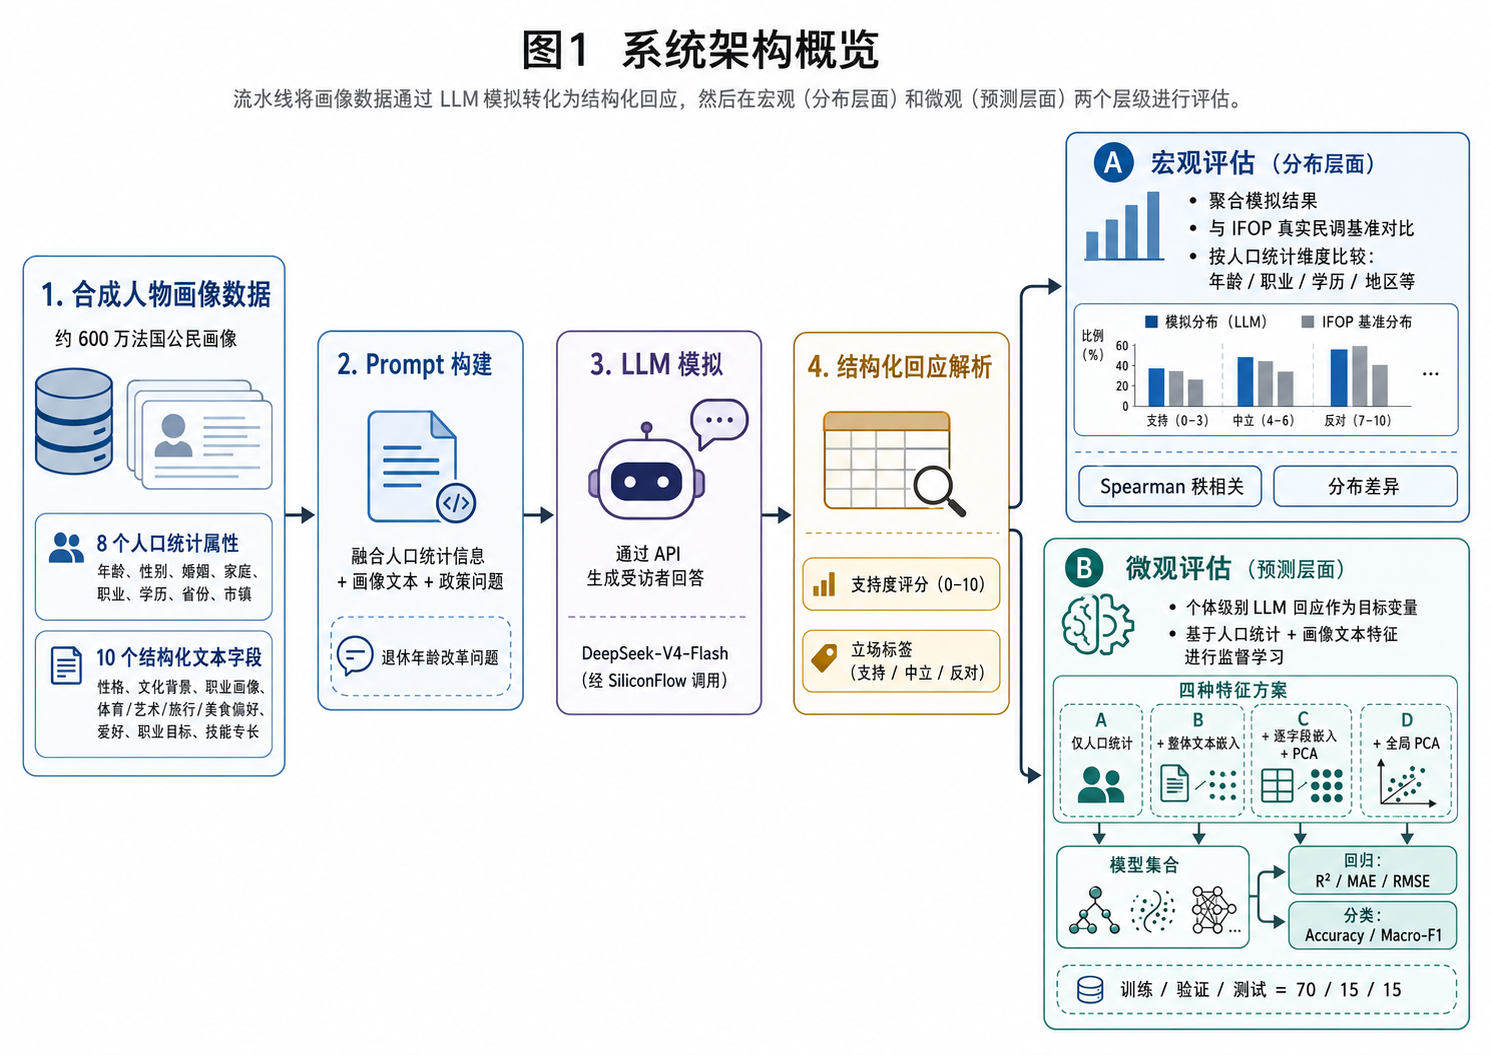
\includegraphics[width=0.85\textwidth]{figures/architecture.png}
    \caption{系统架构概览。流水线将画像数据通过LLM模拟转化为结构化回应，然后在宏观（分布层面）和微观（预测层面）两个层级进行评估。}
    \label{fig:architecture}
\end{figure}

\subsection{人物画像生成}

每个合成的法国公民由18个属性描述，横跨五个类别：基础人口统计（年龄、性别）、社会经济地位（职业、学历、婚姻状况、家庭类型）、地理位置（省份、市镇）、个性轮廓（性格特质、文化背景、职业画像）、生活方式（体育、艺术、旅行、美食、爱好、职业目标、技能专长）。完整数据集约含600万独立画像，以Parquet格式存储（4.2 GB）。

\subsection{Prompt工程：三轮迭代}

我们进行了三轮系统化的Prompt迭代实验，每次向10,000个画像查询相同的退休改革问题：

\begin{quote}
    关于法定退休年龄，您认为应该怎么做？回到62岁、维持在64岁，还是进一步提高？
\end{quote}

表~\ref{tab:prompt_iterations}总结了三轮迭代的关键差异及其与IFOP基准的对比结果。

\begin{table}[H]
    \centering
    \caption{Prompt迭代对比及与IFOP基准的对齐程度}
    \label{tab:prompt_iterations}
    \begin{tabular}{@{}lcccc@{}}
        \toprule
        & \textbf{Run 1} & \textbf{Run 2} & \textbf{Run 3} & \textbf{IFOP} \\
        \midrule
        \textbf{Prompt设计要素} & & & & \\
        \quad 画像引导方式 & 结合自身画像 & +法国形势理解 & 严格基于画像 & --- \\
        \quad 中立规避指令 & 有 & --- & --- & --- \\
        \quad 分数区间映射 & 无 & 无 & 有（0--10） & --- \\
        \quad 示例提供 & 是 & 是 & 否 & --- \\
        \midrule
        \textbf{结果（\%）} & & & & \\
        \quad 回到62岁 & 89.0 & \textbf{72.8} & 28.9 & 61 \\
        \quad 维持64岁 & $\sim$10 & 17.9 & 70.9 & 34 \\
        \quad 进一步提高 & $\sim$1 & 9.3 & 0.1 & 5 \\
        \midrule
        \quad 与IFOP差距 & +28.0 pp & \textbf{+11.8 pp} & $-$32.1 pp & 0 \\
        \quad 平均得分（0--10） & 6.87 & 6.29 & 5.78 & --- \\
        \bottomrule
    \end{tabular}
\end{table}

Run 2取得了最接近真实调查数据的结果。其关键设计要素为：(a) 要求模型结合当前法国形势理解，同时摒弃内置价值观；(b) 保留具体示例以锚定回答格式；(c) 移除明确的"避免中立"指令（该指令在Run 1中推动回答走向极端）。Run 3矫枉过正——同时移除示例和形势背景指令，导致回答坍塌至中立中间地带。

\subsection{LLM模拟设置}

所有实验以Run 2的Prompt模板为基准。LLM API（DeepSeek-V4-Flash）通过SiliconFlow调用，temperature=0.7。每条回答经解析提取数值支持度评分（0--10，回归时缩放到0--1）和三分立场标签（支持/中立/反对）。最终数据集包含8个人口统计特征、10个文本字段和2个目标变量。

\subsection{采样策略：相似度检索与随机抽样}

为检验采样方式对LLM态度模拟的影响，本文设置了两种对照策略：

\begin{enumerate}[leftmargin=*]
    \item \textbf{相似度检索（Similarity-based）：}使用FAISS对画像文本的SBERT嵌入进行语义检索，选取与退休改革问题嵌入余弦相似度最高的前K个画像。该策略筛选出画像描述中与退休、工作、年龄等议题语义相关的个体，效果上可类比传统调查中的"筛选问题"。
    \item \textbf{随机抽样（Random）：}从全部600万画像中均匀随机抽取K个，不施加任何议题相关性约束，作为无信息先验的对照基线。
\end{enumerate}

两种策略使用完全相同的问卷题目、Prompt模板（Run 2）和API参数，K均设为10,000，仅采样方式不同。

\subsection{ML特征与模型}

为从个体层面检验LLM态度输出的可预测性，我们构建了四种特征方案：\textbf{A}（仅8个人口统计特征，标签编码）；\textbf{B}（A + 整段persona\_text的SBERT嵌入，8+384d）；\textbf{C}（A + 10个文本字段各自嵌入后逐字段PCA至16d并拼接，8+160d）；\textbf{D}（A + 10个字段嵌入全拼接3840d后全局PCA至128d）。所有文本嵌入使用\texttt{all-MiniLM-L6-v2}（384维Sentence-BERT）。方案A为纯人口统计基线，方案B为原始实现，方案C和D旨在保留字段级别的语义差异。回归模型涵盖线性模型、集成树（Random Forest/XGBoost/LightGBM/CatBoost）、SVR和MLP共11种；分类模型6种（逻辑回归/朴素贝叶斯/决策树/随机森林/XGBoost/LightGBM），均使用类别权重处理不平衡分布。完整模型配置与超参数见附录。

\subsection{评估协议}

数据按70/15/15划分为训练集/验证集/测试集，在立场标签上分层抽样。四种方案共享完全相同的划分索引以保证公平对比。在训练集上使用5折交叉验证进行模型选择，在留出的测试集上报告最终指标。回归指标：R$^2$、MAE、RMSE；分类指标：准确率和Macro F1。

% ================================================================
\section{结果}
% ================================================================

\subsection{Prompt的威力：从89\%到29\%}

三轮Prompt实验（表~\ref{tab:prompt_iterations}）揭示了LLM态度模拟对措辞选择的极端敏感性。将Run 1与Run 3对比，支持"回到62岁"的比例从89\%骤降至29\%——三轮实验之间，仅Prompt措辞的变化就引发了\textbf{60个百分点的支持率跨度}。作为参照，真实世界中法国退休改革的民意波动——历经数月的全国罢工、媒体辩论和政治博弈——也仅在10--15个百分点范围内波动。换言之，改变一段Prompt可以产生比一场全国性社会运动更大的态度分布偏移。

逐轮分析揭示了各Prompt要素的边际效应。Run 1使用了"避免中立"指令，导致89\%的回答集中在"支持"端，中立和反对几乎被完全压制。去除该指令并加入"结合当前法国形势理解"后（Run 2），分布显著向中间靠拢（支持72.8\%，中立17.9\%），与IFOP的差距从+28pp缩小至+11.8pp。进一步同时移除回答示例和形势背景（Run 3），回答大面积坍塌至中立（70.9\%），支持率降至29\%——尽管问题本身是一个具有明确价值立场的选择题。这一坍塌模式暗示：LLM在缺少示例锚定和情境约束时，倾向于退回"安全"的中立表达。

\subsection{与IFOP的对齐与错位}

Run 2在聚合层面取得了与IFOP最接近的分布（差距+11.8pp），但进一步按CSP职业分类拆解后，对齐质量呈现显著的群体差异（表~\ref{tab:occupation_compare}）。

\begin{table}[H]
    \centering
    \caption{LLM模拟与IFOP调查的CSP职业分类对比（支持"回到62岁"的百分比）}
    \label{tab:occupation_compare}
    \begin{tabular}{@{}lccc@{}}
        \toprule
        \textbf{CSP职业类别} & \textbf{IFOP (\%)} & \textbf{LLM Run 2 (\%)} & \textbf{偏差 (pp)} \\
        \midrule
        Ouvriers（工人） & 73 & 61.4 & $-$11.6 \\
        Employés（雇员） & 77 & 49.8 & $-$27.2 \\
        Professions intermédiaires（中级职业） & 65 & 37.5 & $-$27.5 \\
        Cadres et prof. int. sup.（高管/高级知识分子） & 54 & 31.9 & $-$22.1 \\
        \bottomrule
    \end{tabular}
\end{table}

两个维度的偏差值得注意。其一，\textbf{内部排序存在反转}：IFOP数据中支持度最高的是雇员（77\%），其次为工人（73\%）；而LLM模拟中工人（61.4\%）超过了雇员（49.8\%），提示LLM可能内化了"工人=更激进支持退休年龄降低"的刻板印象，而低估了雇员群体的真实不满程度。其二，\textbf{LLM在所有职业类别上系统性低估了支持度}，偏差幅度在-12至-28pp之间。一个结构性原因是样本构成偏差：LLM相似度检索数据中56.6\%的个体属于CSP分类中的"无职业活动者"（Autres sans activité professionnelle），该类别在IFOP的CSP交叉表中无直接对应项，且在LLM模拟中支持度高达95.6\%，严重拉高了整体均值而掩盖了各职业类别内部的分化。

需要指出的是，"基准"本身并非无偏。IFOP调查（n=2,023）采用在线自填问卷，其CSP分类是一种统计建构，抽样配额、无回答偏差和社会期望偏差均可能影响职业分组数据的准确性。因此，LLM—IFOP差距不应被简单地等同于"LLM的误差"，两个测量体系各有自身的测量不确定性。

\subsection{谁来回答：相似度检索 vs. 随机抽样}

作为方法对照，我们测试了不使用语义筛选的随机抽样（表~\ref{tab:sampling_comparison}）。

\begin{table}[H]
    \centering
    \caption{相似度检索与随机抽样的立场分布对比}
    \label{tab:sampling_comparison}
    \begin{tabular}{@{}lccc@{}}
        \toprule
        & \textbf{IFOP基准} & \textbf{相似度检索} & \textbf{随机抽样} \\
        \midrule
        支持（回到62岁） & 61\% & 72.8\% & 43.4\% \\
        中立（维持64岁） & 34\% & 17.9\% & 37.2\% \\
        反对（进一步提高） & 5\% & 9.3\% & 19.5\% \\
        \midrule
        与IFOP差距（支持率） & --- & +11.8 pp & -17.6 pp \\
        \bottomrule
    \end{tabular}
\end{table}

结果呈现了一个反直觉的规律：直觉上，随机抽样应更接近"无偏"的人口分布，然而其与IFOP基准的差距（-17.6pp）反而大于相似度检索（+11.8pp）。更均衡的分布（支持/中立/反对=43\%/37\%/20\%）并未带来更准确的基准对齐。

这一现象的背后机制是：退休改革是一个有明确利益相关群体的议题。随机抽样大量纳入了与退休毫无语义关联的个体（如20岁学生、全职家长），LLM在面对此类画像时缺乏角色扮演的语义锚点，其回答更接近"猜测"而非"推理"，从而导致分布偏离真实利益相关者的态度。相似度检索虽引入了对"议题相关者"的选择偏倚，但这一偏倚恰好与传统调查中筛选问题（screening question）的功能一致——在测量态度之前，先锁定议题相关的子群体。这提示：\textbf{LLM民调中"代表性"的内涵可能需要从人口统计均衡转向语义相关性}。

\subsection{年龄压倒一切：个体层面的特征分析}

为理解哪些特征在驱动LLM的个体态度输出，我们使用SHAP对方案C（人口统计+逐字段PCA）的XGBoost回归模型进行了特征重要性分析（图~\ref{fig:feature_importance}）。方案C被选中分析的原因是其字段名前缀（如persona\_pc*）使每个PCA分量可追溯至原始文本字段，便于语义解释。

\begin{figure}[H]
    \centering
    \begin{subfigure}{0.48\textwidth}
        \centering
        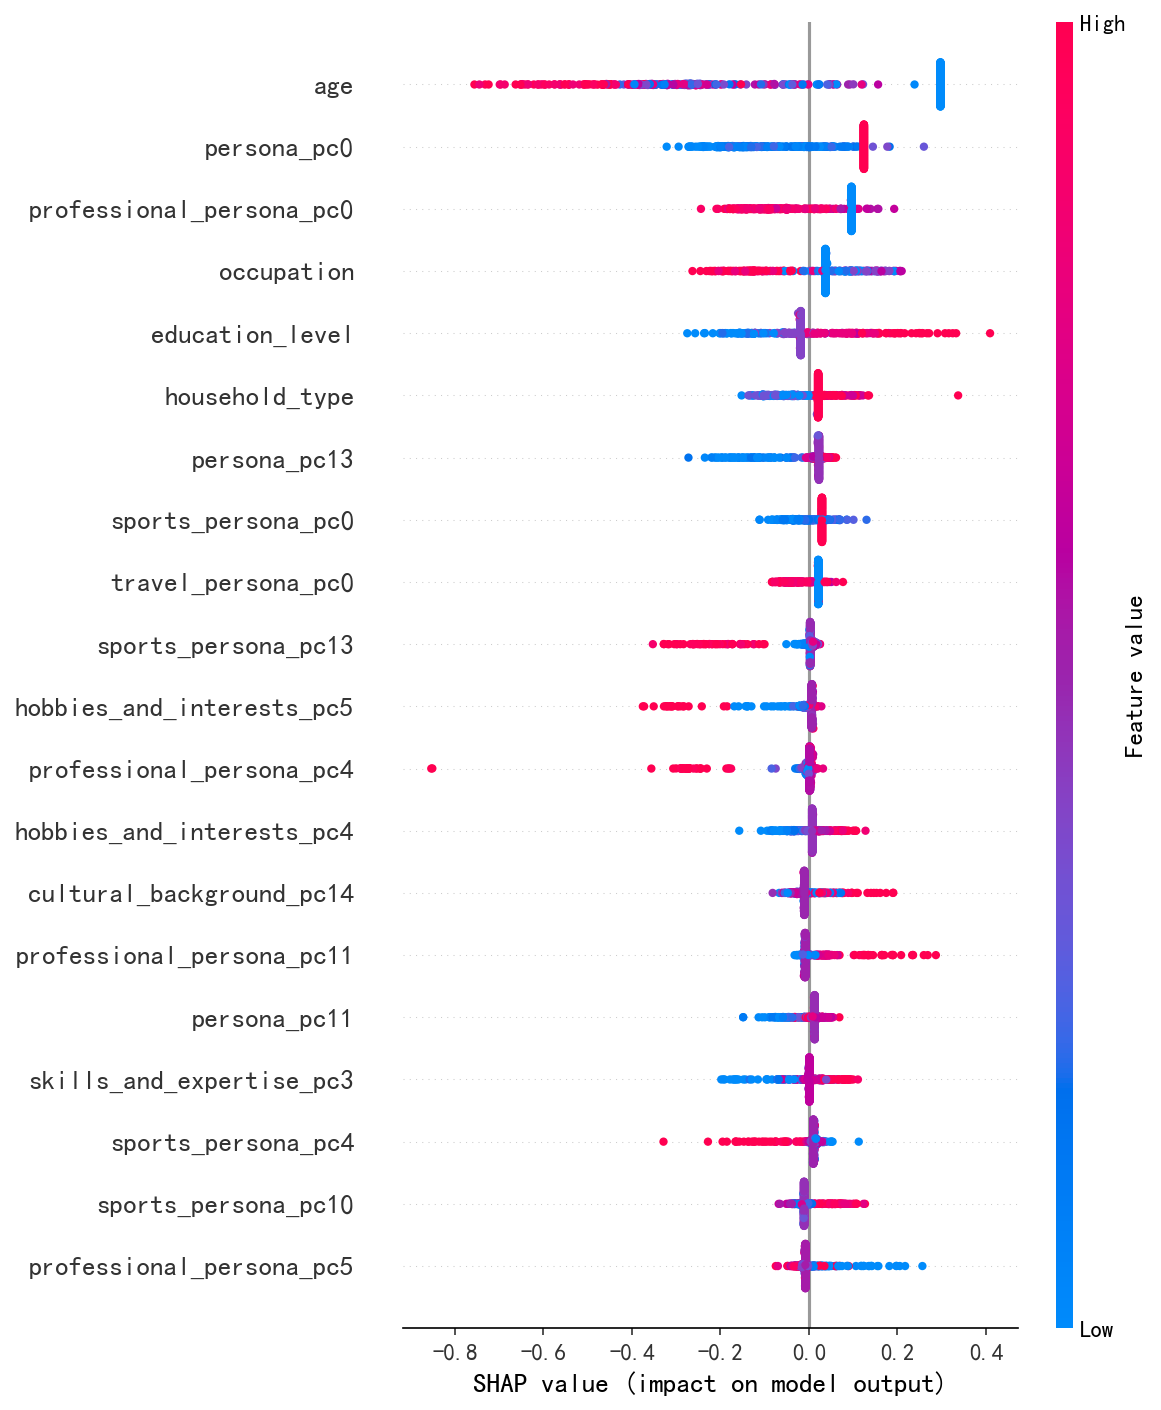
\includegraphics[width=\textwidth]{figures/shap_summary.png}
        \caption{SHAP概要图}
        \label{fig:shap_summary}
    \end{subfigure}
    \hfill
    \begin{subfigure}{0.48\textwidth}
        \centering
        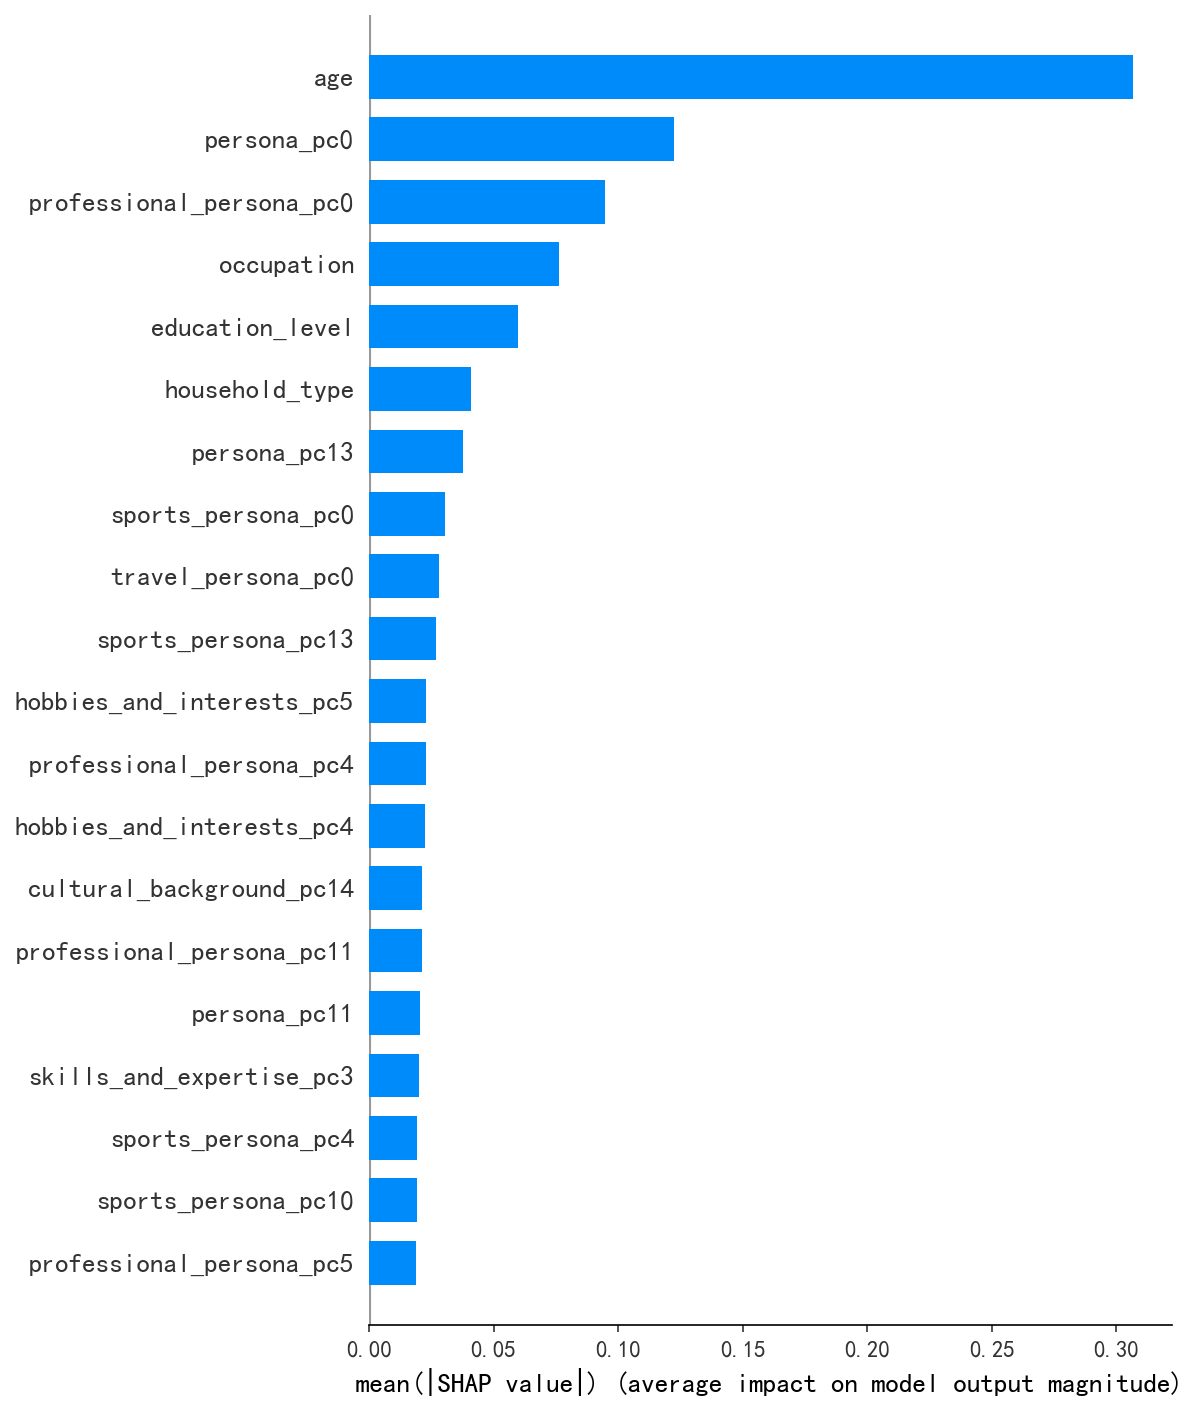
\includegraphics[width=\textwidth]{figures/shap_bar.png}
        \caption{SHAP柱状图}
        \label{fig:shap_bar}
    \end{subfigure}
    \caption{方案C（人口统计+逐字段PCA）XGBoost回归模型的SHAP特征重要性分析。}
    \label{fig:feature_importance}
\end{figure}

SHAP分析呈现了一个极为清晰的信号结构：\textbf{年龄（age）}是唯一具有实质预测力的特征（$|$SHAP$|$=0.307），远超其他所有变量。这与法国退休改革的社会现实高度一致——退休年龄的变动对不同年龄群体的利益影响截然不同：临近退休者与刚入职场的年轻人的计算逻辑完全不同。排名第二、第三的persona\_pc0（$|$SHAP$|$=0.122）和professional\_persona\_pc0（$|$SHAP$|$=0.095）仅约为年龄贡献的三分之一，表明性格特质和职业画像的语义整体方向携带了少量态度信号。

从宏观格局看，8个人口统计特征合计贡献了总SHAP量的24\%，160个文本PCA分量合计贡献了76\%。然而文本信号的分布高度分散——单个文本PCA分量的平均$|$SHAP$|$仅约0.01，不足任何单个人口统计特征的十分之一。这解释了后续R$^2$分析的发现：文本嵌入虽然在总量上携带了态度相关信息，但这些信号分散在大量弱特征中，无法汇聚成超越少数强人口统计特征的预测增量。在文本字段内部，persona（性格特质）和professional\_persona（职业画像）的分量出现在Top-15中的频率最高，而travel\_persona、culinary\_persona等生活方式字段排名靠后，暗示与政策态度更相关的语义维度集中在个人核心自我定位的描述中，而非具体的消费或兴趣偏好。SHAP依赖图（附录图~\ref{fig:shap_dependence}）进一步确认了年龄与预测支持度之间的负相关关系。

\subsection{R$^2\approx 0.28$的天花板}

四种特征方案的回归和分类结果（表~\ref{tab:regression_best}和~\ref{tab:classification_best}）指向同一个结论：\textbf{所有道路通向同一天花板}。

\begin{table}[H]
    \centering
    \caption{各方案最佳回归模型（测试集）}
    \label{tab:regression_best}
    \begin{tabular}{@{}lcccc@{}}
        \toprule
        \textbf{方案} & \textbf{最佳模型} & \textbf{Test R$^2$} & \textbf{MAE} & \textbf{RMSE} \\
        \midrule
        D（+全局PCA） & Random Forest & 0.284 & 0.77 & 1.26 \\
        A（仅人口统计） & CatBoost & 0.273 & 0.76 & 1.27 \\
        B（+persona\_text） & CatBoost & 0.272 & 0.77 & 1.27 \\
        C（+逐字段PCA） & CatBoost & 0.271 & 0.77 & 1.27 \\
        \bottomrule
    \end{tabular}
\end{table}

\begin{table}[H]
    \centering
    \caption{各方案最佳分类模型（测试集）}
    \label{tab:classification_best}
    \begin{tabular}{@{}lcccc@{}}
        \toprule
        \textbf{方案} & \textbf{最佳模型} & \textbf{Acc} & \textbf{Macro F1} \\
        \midrule
        A（仅人口统计） & Random Forest & 0.714 & 0.507 \\
        C（+逐字段PCA） & XGBoost & 0.704 & 0.504 \\
        B（+persona\_text） & LightGBM & 0.723 & 0.489 \\
        D（+全局PCA） & Random Forest & 0.724 & 0.446 \\
        \bottomrule
    \end{tabular}
\end{table}

回归方面，四种方案的Test R$^2$被压缩在0.271--0.284的极窄区间内，方案间最大差异不足0.015。即便是表现最好的方案D（R$^2$=0.284），相比纯人口统计基线（方案A，R$^2$=0.273）也仅有约0.01的提升——10个文本字段、3840维SBERT嵌入、精心设计的PCA降维策略，合计贡献了相当于约1\%的额外可解释方差。分类任务呈现相同模式：Macro F1集中在0.446--0.507的窄区间，方案A（仅人口统计）反而取得最佳（0.507），方案D在分类上表现最差（0.446），提示全局PCA虽然保留了连续方差信号，但平滑了离散类别边界。

学习曲线（图~\ref{fig:learning_curves}）为这一天花板提供了进一步的证据：四个方案均在约3,500个训练样本后收敛，验证集R$^2$进入平台期，继续增加数据几乎不带来增益。训练集与验证集之间存在持续且不可缩小的R$^2$差距，说明天花板不是数据量不足，而是信号噪声比的根本性限制。

\begin{figure}[H]
    \centering
    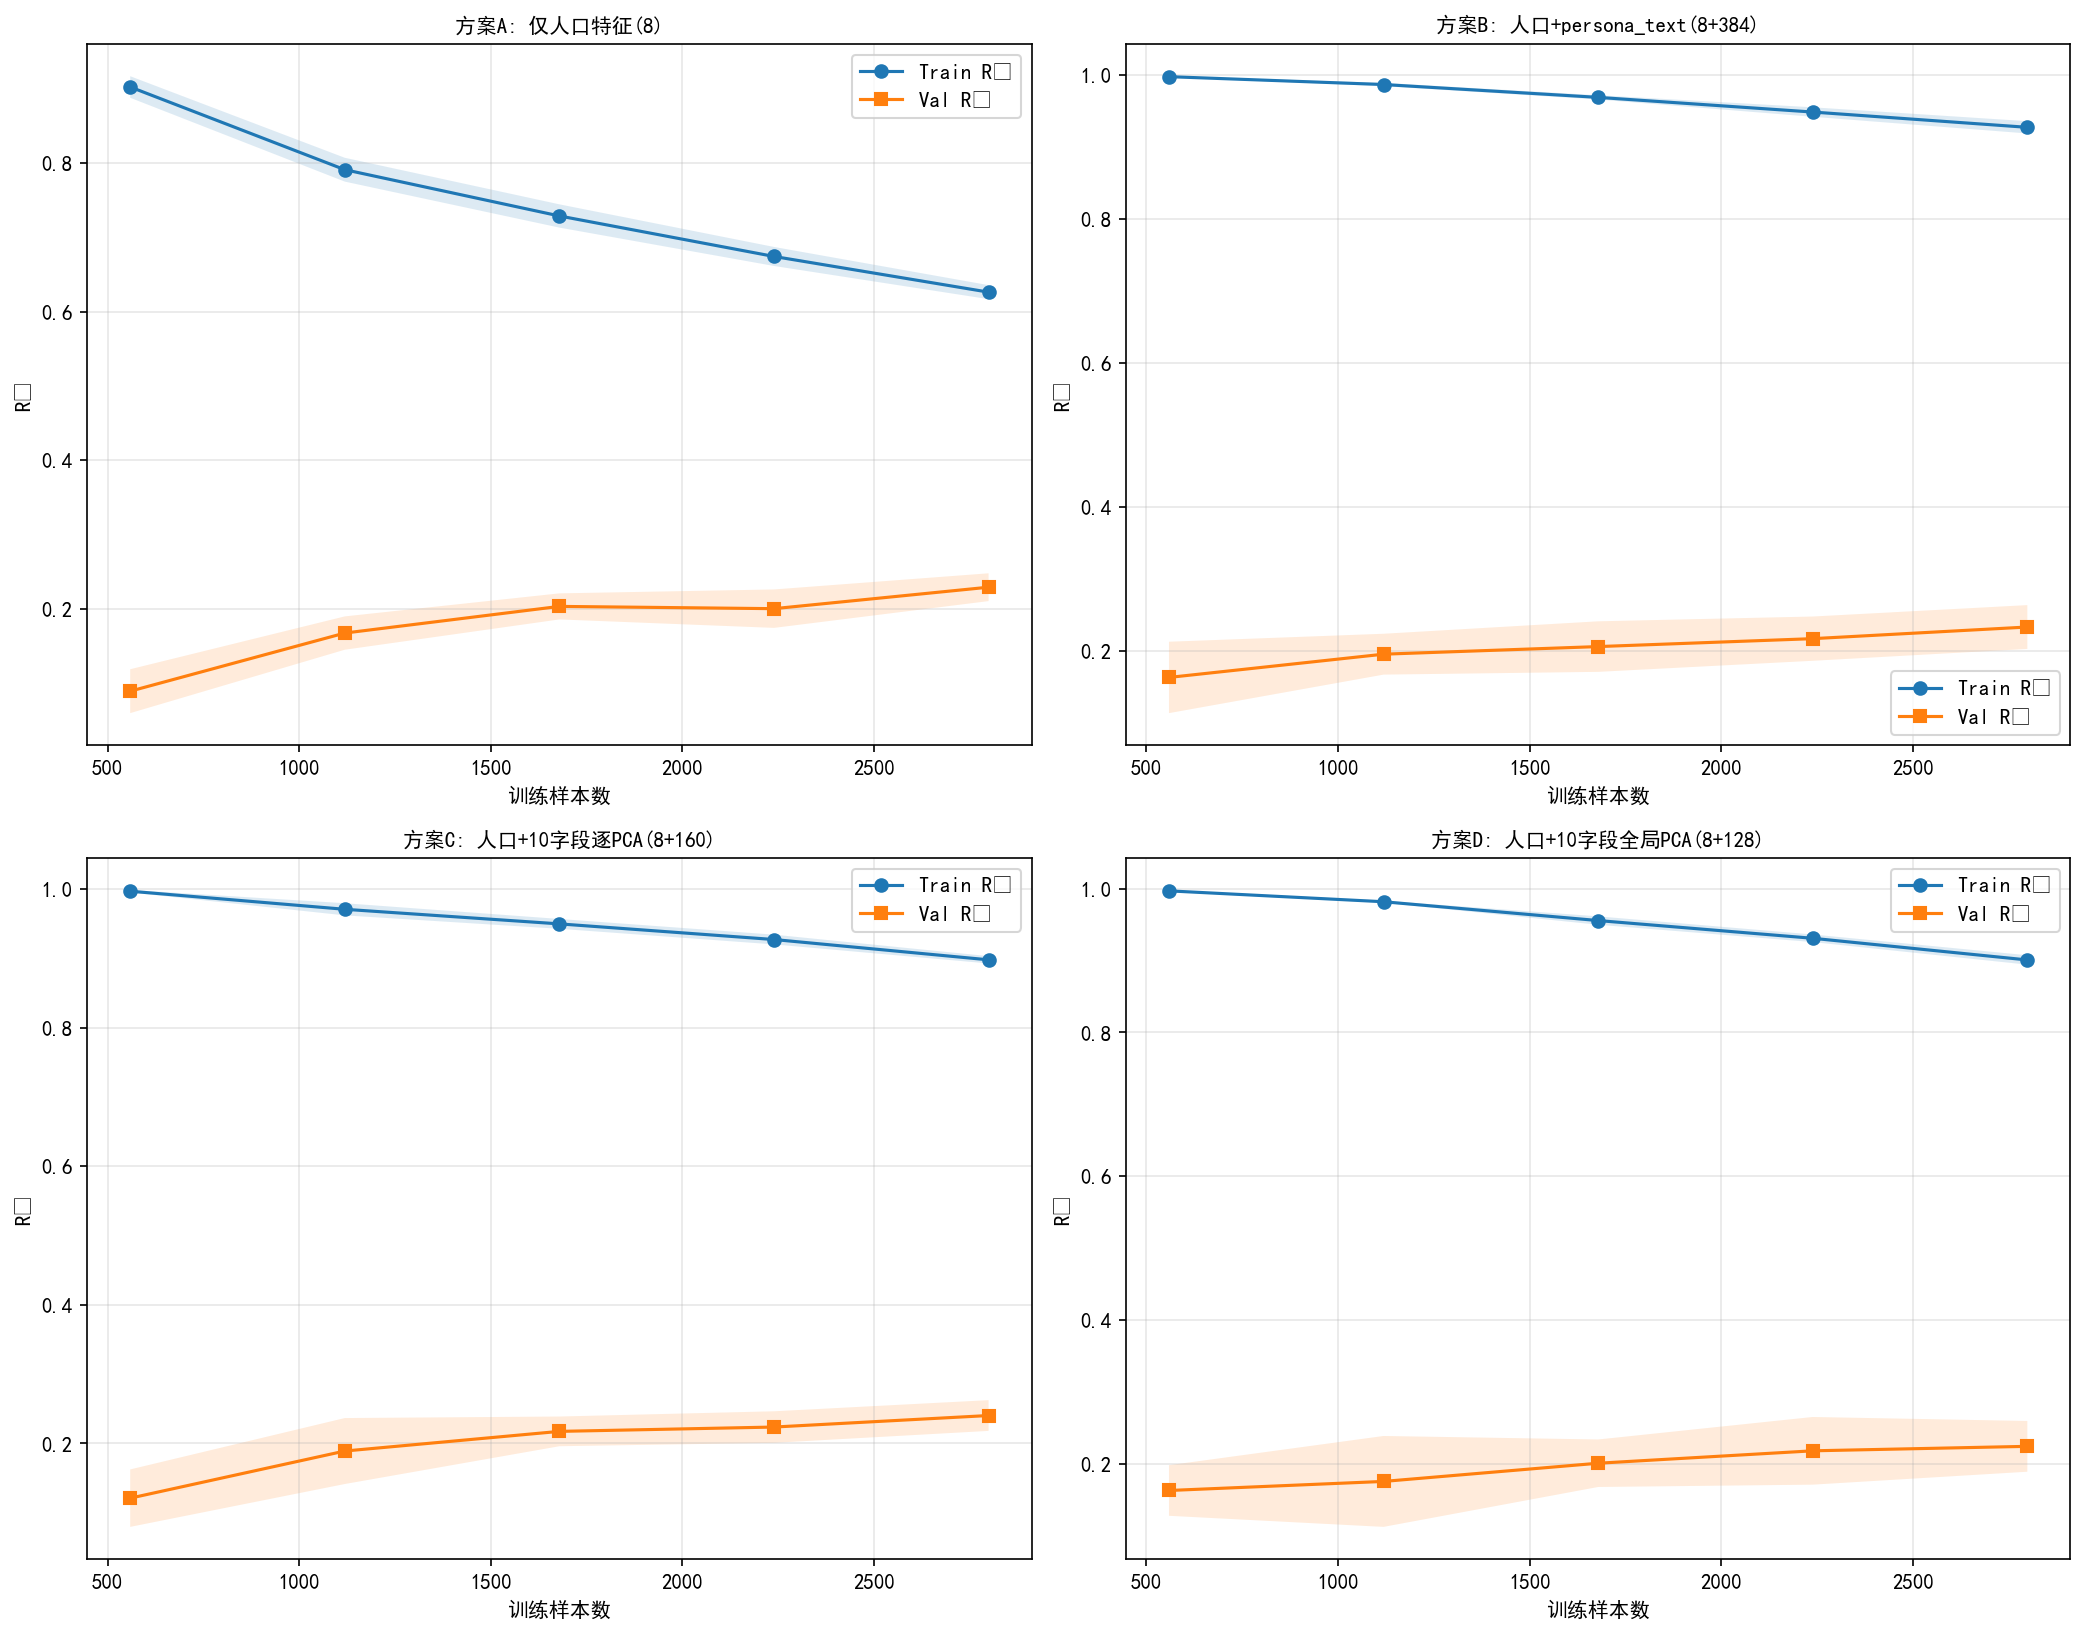
\includegraphics[width=0.95\textwidth]{figures/learning_curves.png}
    \caption{四种特征方案的学习曲线（2$\times$2）。所有方案在相近的验证集R$^2$水平上收敛。}
    \label{fig:learning_curves}
\end{figure}

形式化而言，将LLM支持度评分分解为$y_i = f(x_i) + \epsilon_i$，其中$f(x_i)$为画像特征与态度之间的系统性关系，$\epsilon_i$为LLM在$T=0.7$下的采样噪声，则R$^2 \approx 0.28$意味着$\text{Var}(\epsilon) \approx 2.6 \times \text{Var}(f(x))$——\textbf{LLM的随机波动约为画像特征系统性变异的2.6倍}。换言之，即使同一个人物画像被重复询问，LLM给出的支持度分数也会因采样温度而产生非平凡方差，这一噪声基底是任何特征工程都无法克服的。

% ================================================================
\section{讨论}
% ================================================================

\subsection{Prompt敏感性：工具与风险}

三轮Prompt实验中最引人注目的发现——60个百分点的支持率跨度——既是LLM民调的有力工具，也是其重要风险。\textbf{作为工具}，Prompt工程可以显著改善模拟分布与真实基准的对齐质量：Run 2通过精准的设计选择（移除中立规避、加入形势理解、保留示例锚定），将差距从+28pp缩小至+12pp，效果显著。\textbf{作为风险}，Prompt敏感性意味着研究者的自由度极大——不同的Prompt措辞选择可以产生几乎任意的分布结果。这要求在LLM民调研究中，Prompt设计必须被充分报告且作为方法学变量的组成部分接受系统检验，而非被视作隐性的"默认设置"。我们建议未来研究将Prompt消融分析作为标准实践，正如传统调查中需要报告问卷措辞和题序效应一样。

\subsection{"代表性"的再定义}

相似度检索与随机抽样的对比结果挑战了LLM民调中关于"代表性"的一项隐含假设。传统调查追求人口统计学意义上的代表性——随机抽样是其黄金标准。然而，本文的实证结果表明：在LLM模拟场景中，随机抽样产生了与真实基准\textit{偏差更大}的分布。其根本原因在于，LLM的角色扮演并非在所有画像上表现一致——当画像与议题之间缺乏语义关联时，LLM的"角色扮演"退化为"猜测"，其回答不再反映画像特征与议题之间的任何系统性关系。在这种情况下，人口统计学上的"代表性"实际上意味着大量不相关回答的平均，反而稀释了有意义的态度信号。

我们因此主张：LLM民调的"代表性"应至少包含两个维度——人口统计均衡\textit{和}语义相关性。相似度检索不应被视为"引入偏差"的技术缺陷，而应理解为一种主动的样本设计策略，在方法论上与传统调查的筛选问题、准实验中的受试者遴选具有同构性。关键要求是：研究者必须明确报告采样策略及其对结论适用范围的影响。

\subsection{个体预测的根本限制}

所有特征方案和模型收敛至同一R$^2$天花板（$\approx$0.28）的事实，将问题的焦点从"哪个方案更好"转移到了"为什么存在天花板"。我们的分析指向LLM采样温度所引入的不可约噪声：$T=0.7$下，同一画像的重复回答存在实质性方差，这部分方差与任何可观测特征无关。在分类任务中，即便使用类别权重处理不平衡，Macro F1的天花板（$\approx$0.51）仍远低于实际可用的精度水平。这意味着：在当前LLM范式下，从画像特征出发进行可靠的个体级别政治立场预测尚不可行。降低温度、多次采样取均值、或使用更大的模型可能在一定程度上缓解这一问题，但LLM固有的随机性不太可能被完全消除。

\subsection{局限性}

本研究存在若干局限。第一，仅测试了一项政策议题（退休改革）和一个LLM（DeepSeek-V4-Flash），其他议题或模型可能呈现不同的行为模式。第二，10,000样本量虽足以支撑ML建模，但限制了人口统计子群体分析的统计效力。第三，IFOP基准（n=2,023）本身也存在抽样误差，因此"真实值"具有不确定性。第四，我们未系统变化采样温度，也未测量重测信度——这是量化LLM噪声基底的直接方法。第五，所有Prompt均以中文编写但面向法国人物画像语境，可能引入语言条件效应。

% ================================================================
\section{结论}
% ================================================================

本文通过三轮Prompt消融实验、两种采样策略对照和系统的ML建模，对LLM模拟法国公民政策态度的行为规律进行了实证研究。主要结论如下：

（1）\textbf{Prompt设计对LLM态度模拟具有压倒性影响。}三轮实验之间仅Promp措辞的变化就产生了60个百分点的支持率跨度，其效应量超过真实世界的社会运动。Run 2通过审慎设计（画像依从+形势认知+格式锚定）将分布与IFOP基准的差距压缩至+12pp，证明了Prompt工程在方法论层面的可行性。

（2）\textbf{采样策略显著影响模拟质量，语义筛选优于随机抽样。}相似度检索通过聚焦与议题语义相关的子群体，在聚合分布上比随机抽样更接近真实基准。这一反直觉的发现表明LLM民调的"代表性"不应等同于人口统计均衡，语义相关性至少同等重要。

（3）\textbf{个体层面的态度预测面临硬性天花板。}年龄是唯一具有实质预测力的特征（$|$SHAP$|$=0.307），文本画像嵌入仅提供可忽略不计的额外预测力。所有特征方案和模型收敛至R$^2\approx 0.28$的同一天花板，受限于LLM采样温度引入的不可约噪声。这一发现对将LLM用于个体级别政治分析的应用场景给出了实证约束。

未来工作包括：将框架扩展至更多政策议题以检验跨议题泛化性；系统变化LLM温度参数以量化随机性-噪声关系；引入真实调查微观数据进行个体层面的直接验证；探索基于政治文本微调的专用态度编码器替代通用Sentence-BERT嵌入。

\section*{致谢}
感谢IFOP、ELABE和Odoxa公开其调查数据，感谢SiliconFlow提供DeepSeek-V4-Flash的API访问。

% ── 参考文献 ───────────────────────────────────────────────────
\begin{thebibliography}{20}

\bibitem{groves2009survey}
R.~M. Groves, F.~J. Fowler, M.~P. Couper, J.~M. Lepkowski, E.~Singer, and R.~Tourangeau.
\newblock \textit{Survey Methodology}, 2nd ed. Wiley, 2009.

\bibitem{argyle2023out}
L.~P. Argyle, E.~C. Busby, N.~Fulda, J.~R. Gubler, C.~Rytting, and D.~Wingate.
\newblock Out of one, many: Using language models to simulate human samples.
\newblock \textit{Political Analysis}, 31(3):337--351, 2023.

\bibitem{santurkar2023whose}
S.~Santurkar, E.~Durmaz, F.~Ladhak, C.~Lee, P.~Liang, and T.~Hashimoto.
\newblock Whose opinions do language models reflect?
\newblock In \textit{ICML}, 2023.

\bibitem{park2023generative}
J.~S. Park, J.~C. O'Brien, C.~J. Cai, M.~R. Morris, P.~Liang, and M.~S. Bernstein.
\newblock Generative agents: Interactive simulacra of human behavior.
\newblock In \textit{UIST}, 2023.

\bibitem{barbera2015tweeting}
P.~Barber\'a.
\newblock Birds of the same feather tweet together: Bayesian ideal point estimation using Twitter data.
\newblock \textit{Political Analysis}, 23(1):76--91, 2015.

\bibitem{hersh2015hacking}
E.~D. Hersh.
\newblock \textit{Hacking the Electorate: How Campaigns Perceive Voters}. Cambridge University Press, 2015.

\bibitem{montgomery2018predicting}
J.~M. Montgomery and S.~Olivella.
\newblock Predicting elections with big data.
\newblock In \textit{The Oxford Handbook of Electoral Systems}, 2018.

\bibitem{reimers2019sentence}
N.~Reimers and I.~Gurevych.
\newblock Sentence-BERT: Sentence embeddings using Siamese BERT-networks.
\newblock In \textit{EMNLP-IJCNLP}, 2019.

\bibitem{ifop2025retraites}
IFOP/CGT.
\newblock Les Fran\c{c}ais et la r\'eforme des retraites.
\newblock Technical report, April 2025.

\bibitem{elabe2026}
ELABE/BFMTV.
\newblock L'\'etat d'esprit des Fran\c{c}ais pour 2026.
\newblock Technical report, January 2026.

\end{thebibliography}

% ── 附录 ───────────────────────────────────────────────────────
\appendix
\section{完整回归结果}

\begin{table}[H]
    \centering
    \caption{全部回归模型 $\times$ 全部方案（验证集，按R$^2$降序排列）}
    \label{tab:regression_all}
    \resizebox{\textwidth}{!}{%
    \begin{tabular}{@{}llrrr@{}}
        \toprule
        \textbf{方案} & \textbf{模型} & \textbf{Val R$^2$} & \textbf{Val MAE} & \textbf{5折CV R$^2$} \\
        \midrule
        D & Random Forest & 0.276 & 0.79 & 0.253 $\pm$ 0.036 \\
        C & CatBoost & 0.275 & 0.79 & 0.259 $\pm$ 0.035 \\
        D & CatBoost & 0.271 & 0.79 & 0.256 $\pm$ 0.033 \\
        C & Random Forest & 0.273 & 0.79 & 0.253 $\pm$ 0.034 \\
        B & CatBoost & 0.258 & 0.80 & 0.247 $\pm$ 0.027 \\
        A & CatBoost & 0.252 & 0.79 & 0.258 $\pm$ 0.021 \\
        \bottomrule
    \end{tabular}%
    }
\end{table}

\section{Prompt模板}

\textbf{Run 2（表现最佳）的Prompt：}

\begin{quote}
\small
你是一位法国公民，请根据人物画像回答政策问题。

【基础信息】/【社会背景】/【个人画像】/【兴趣爱好】/【职业发展】
\textit{[此处插入人物画像详细信息]}

【问题】关于法定退休年龄，您认为应该怎么做？回到62岁、维持在64岁，还是进一步提高？

【要求】
1. 第一人称"我"视角
2. 用中文，简短精炼准确
3. 结合自身画像，真实自然
4. 请结合你对当前法国形势的理解，更真实地扮演角色，摒弃你自身内置的价值观，回答需具有实时性
5. 避免过度极端语气，理性客观
6. 结尾标注：支持度：X/10（0-10分）

示例：作为一名45岁男性工人，我认为...支持度：3/10
\end{quote}

\section{可复现性}

所有代码见于项目仓库\texttt{french\_policy\_simulator/}。主要分析流水线可通过以下命令执行：

\begin{verbatim}
python scripts/05_ml_modeling.py
\end{verbatim}

配置参数（RANDOM\_STATE=42, TRAIN\_SIZE=0.70, VAL\_SIZE=0.15, PCA\_DIMS\_PER\_FIELD=16, PCA\_DIMS\_GLOBAL=128）在脚本开头定义。Sentence-BERT模型（\texttt{all-MiniLM-L6-v2}）在本地缓存，支持离线使用。

\section{补充图表}

\begin{figure}[H]
    \centering
    \begin{subfigure}{0.48\textwidth}
        \centering
        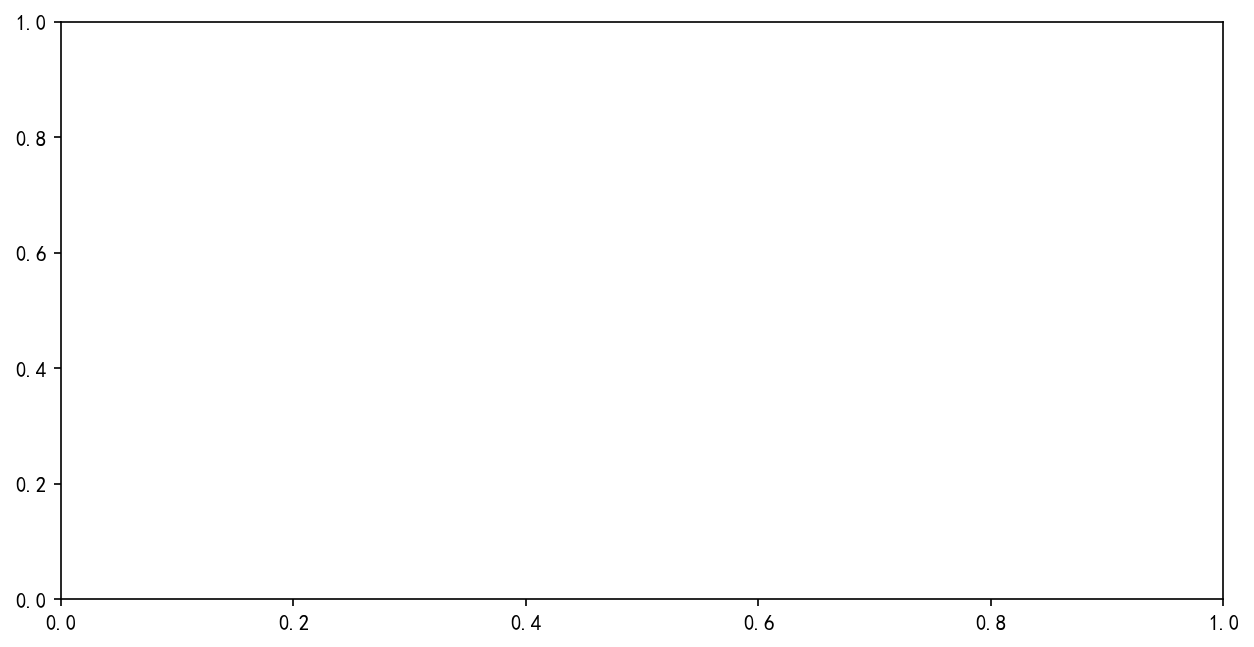
\includegraphics[width=\textwidth]{figures/shap_dependence_1.png}
        \caption{SHAP依赖图：年龄对预测值的影响}
    \end{subfigure}
    \hfill
    \begin{subfigure}{0.48\textwidth}
        \centering
        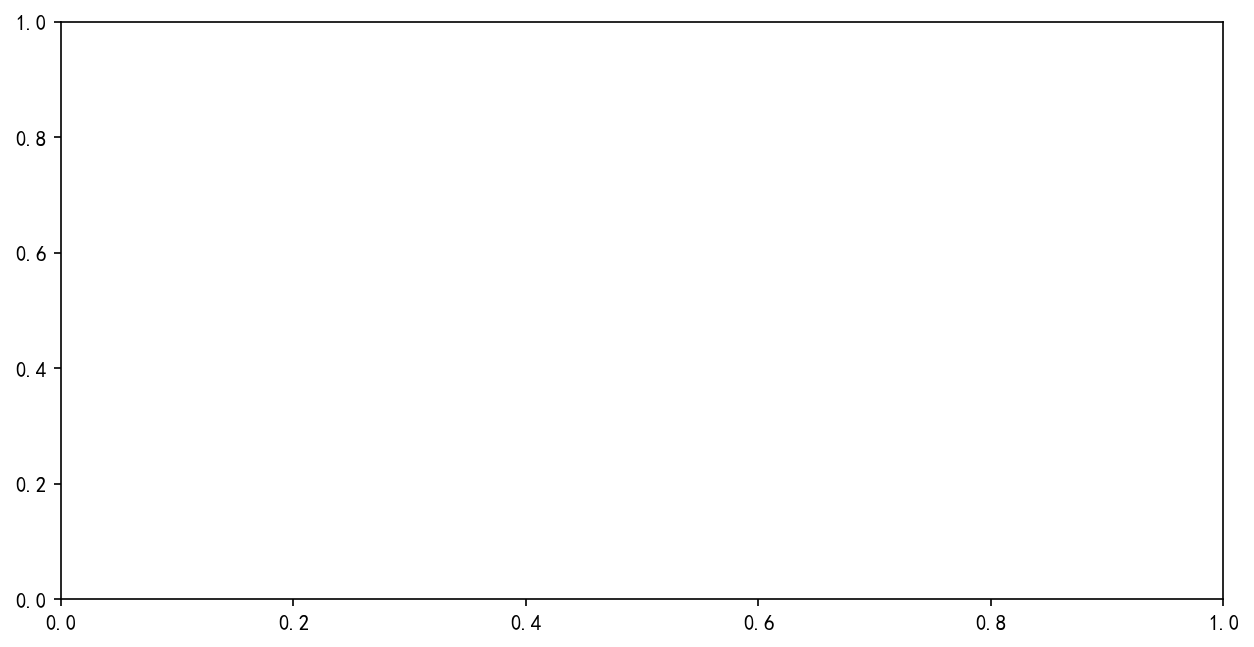
\includegraphics[width=\textwidth]{figures/shap_dependence_2.png}
        \caption{SHAP依赖图：persona\_pc0对预测值的影响}
    \end{subfigure}
    \caption{SHAP依赖图：展示排名前两位的特征（age和persona\_pc0）如何随特征取值变化影响模型预测。年龄与预测支持度呈明显的负相关关系，与法国退休改革的社会现实一致。}
    \label{fig:shap_dependence}
\end{figure}

\begin{figure}[H]
    \centering
    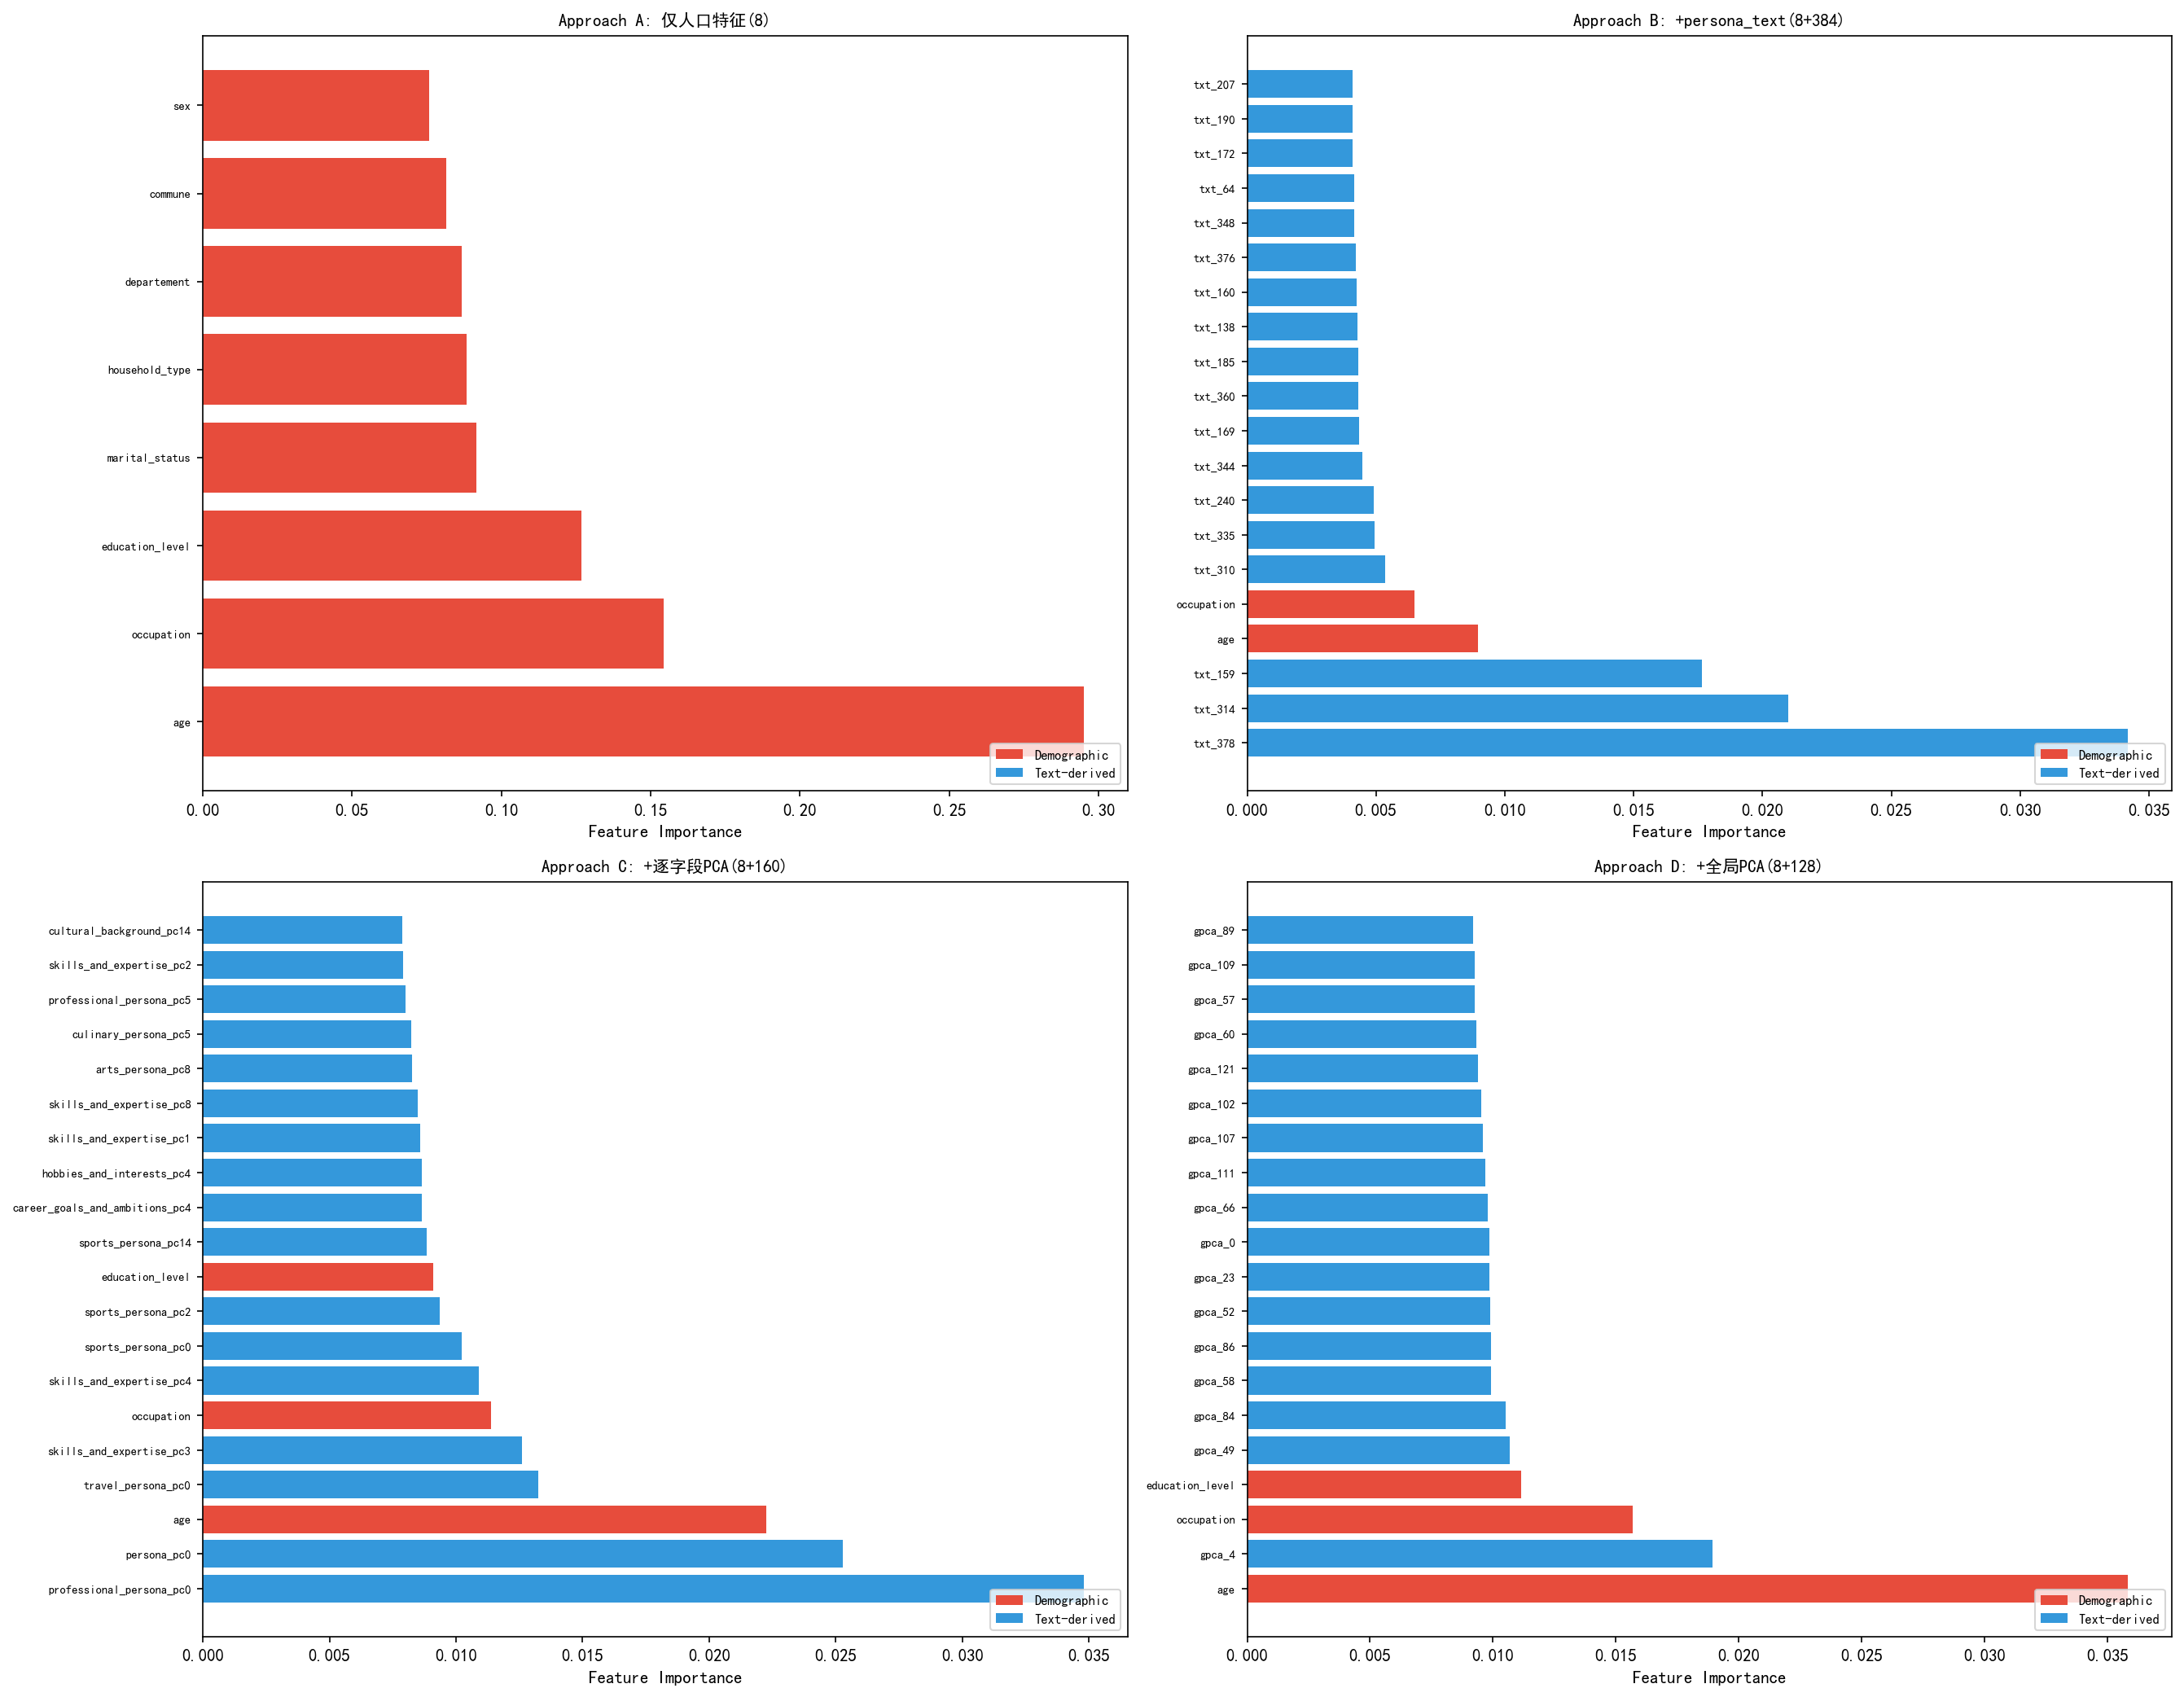
\includegraphics[width=0.95\textwidth]{figures/feature_importance_grid.png}
    \caption{四种方案下XGBoost特征重要性Top-20对比。红色为人口统计特征，蓝色为文本衍生特征。}
    \label{fig:feature_importance_grid}
\end{figure}

\begin{figure}[H]
    \centering
    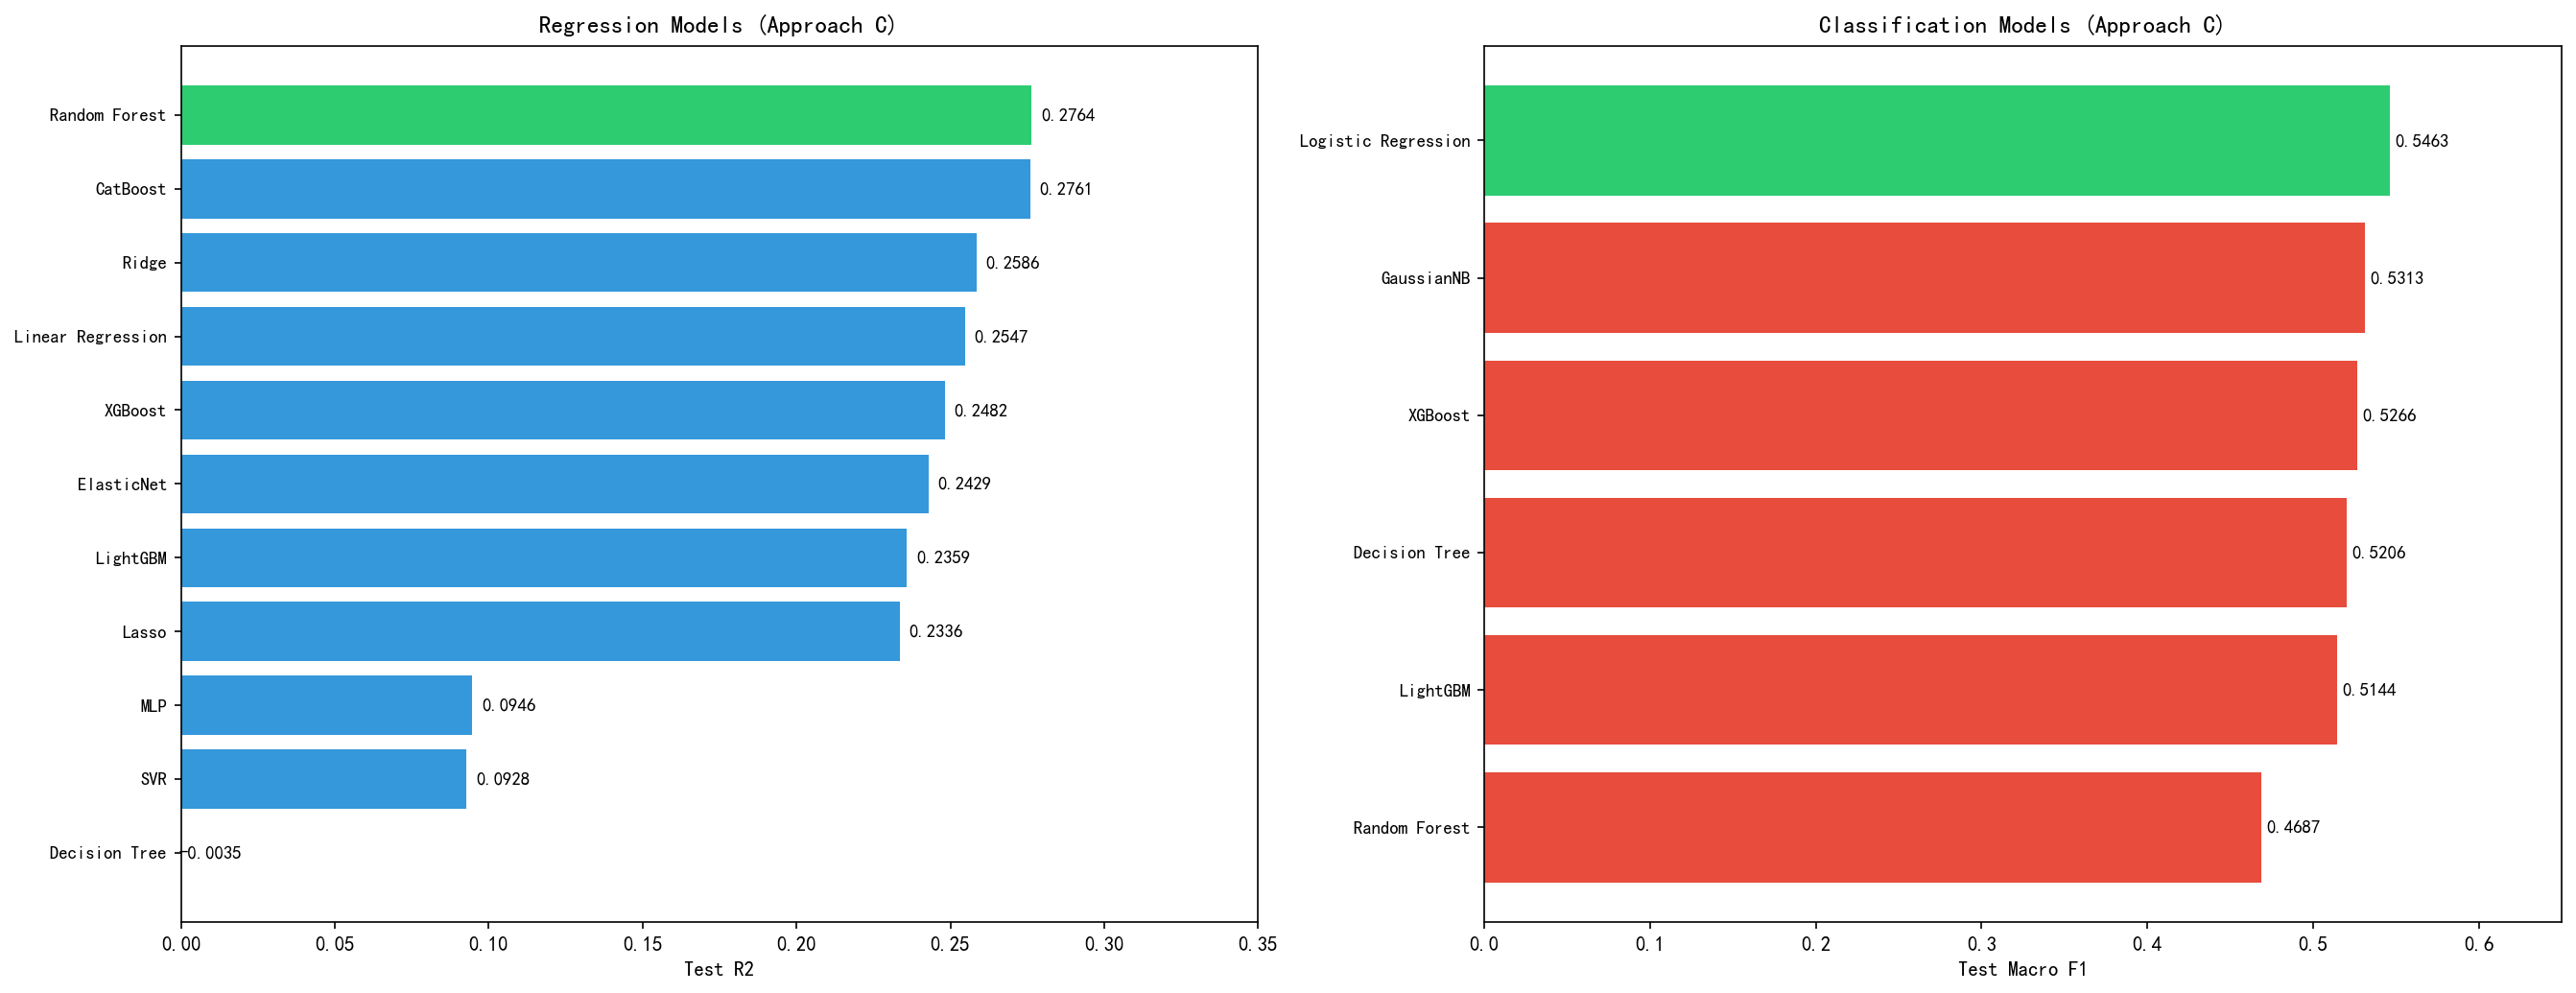
\includegraphics[width=0.95\textwidth]{figures/model_comparison.png}
    \caption{方案C下所有回归模型（左）和分类模型（右）的Test表现排名。}
    \label{fig:model_comparison}
\end{figure}

\begin{figure}[H]
    \centering
    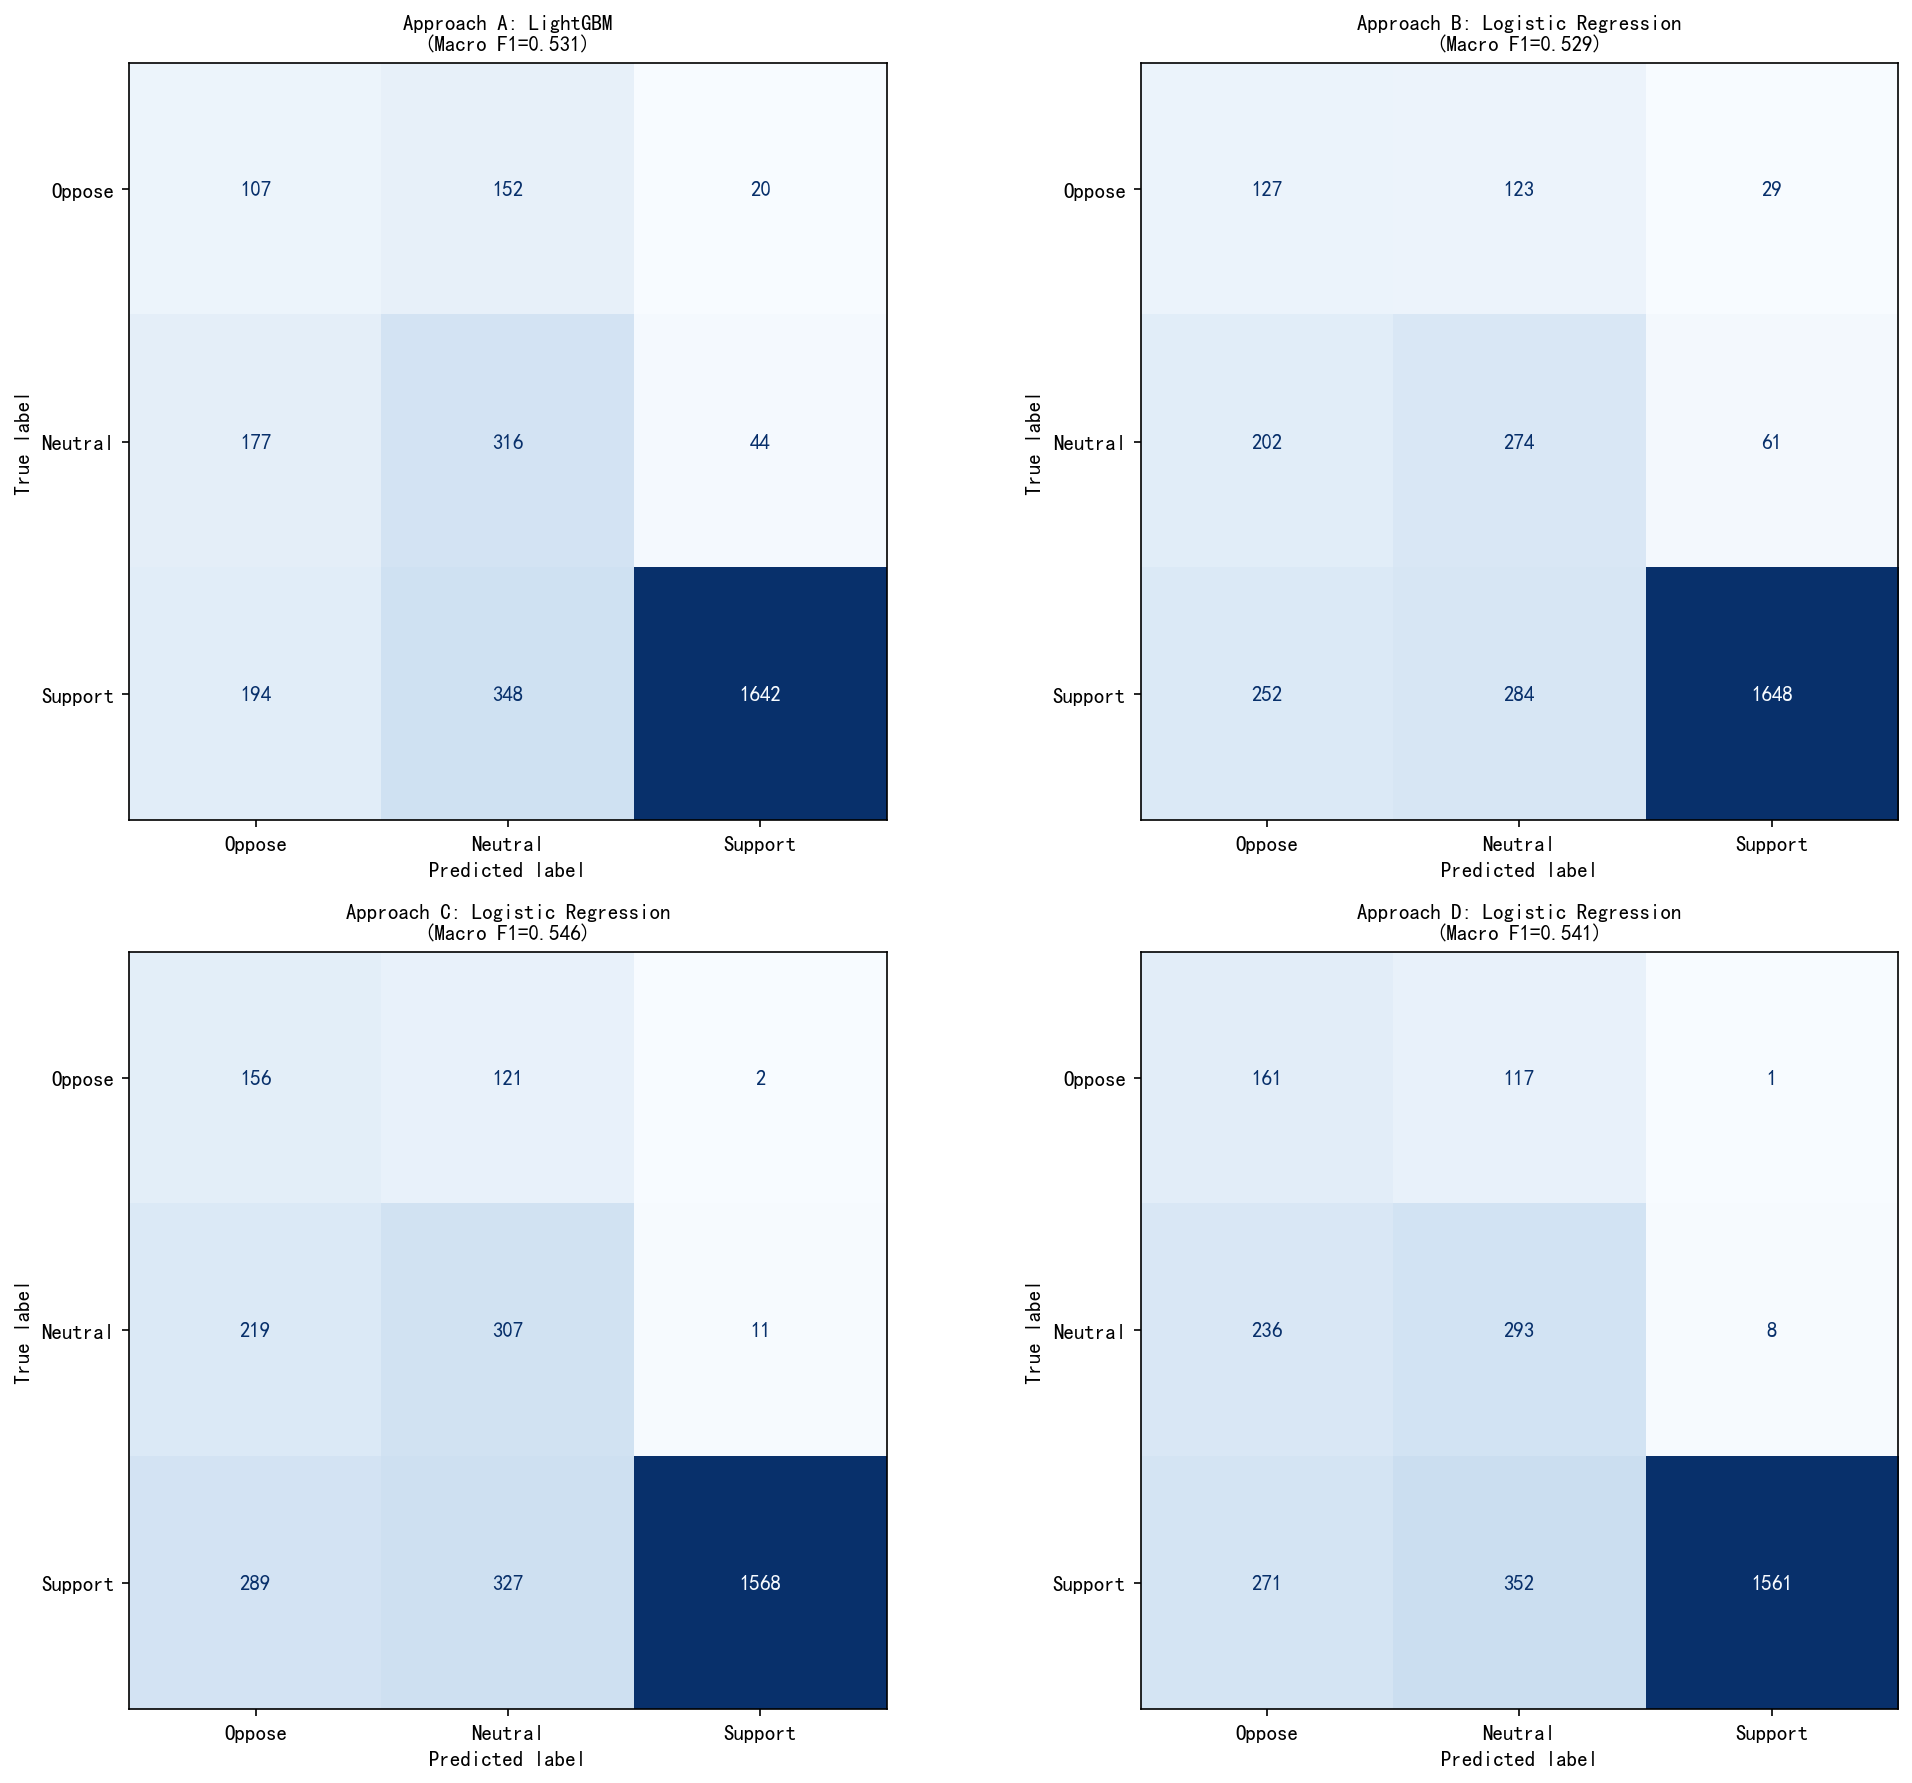
\includegraphics[width=0.95\textwidth]{figures/confusion_matrices.png}
    \caption{四种方案最佳分类模型的混淆矩阵。方案D对"反对"类别的召回率为零。}
    \label{fig:confusion_matrices}
\end{figure}

\begin{figure}[H]
    \centering
    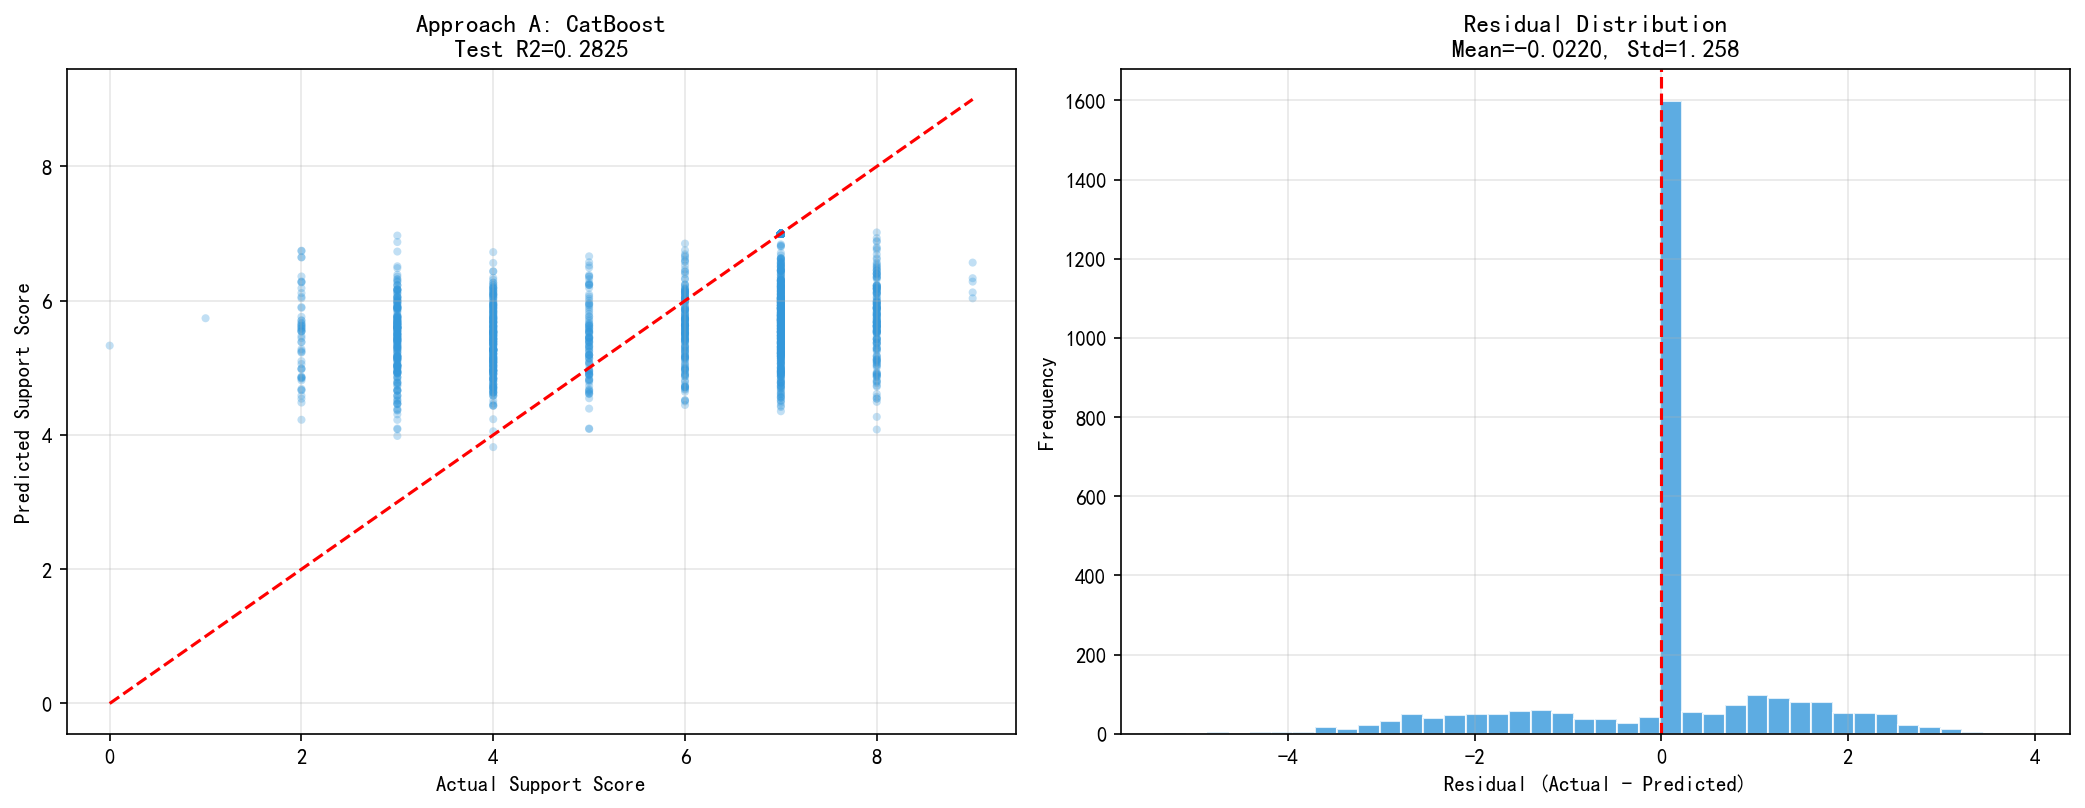
\includegraphics[width=0.95\textwidth]{figures/actual_vs_predicted.png}
    \caption{最优回归模型的预测值与真实值对比（左）及残差分布（右）。}
    \label{fig:actual_vs_predicted}
\end{figure}

\begin{figure}[H]
    \centering
    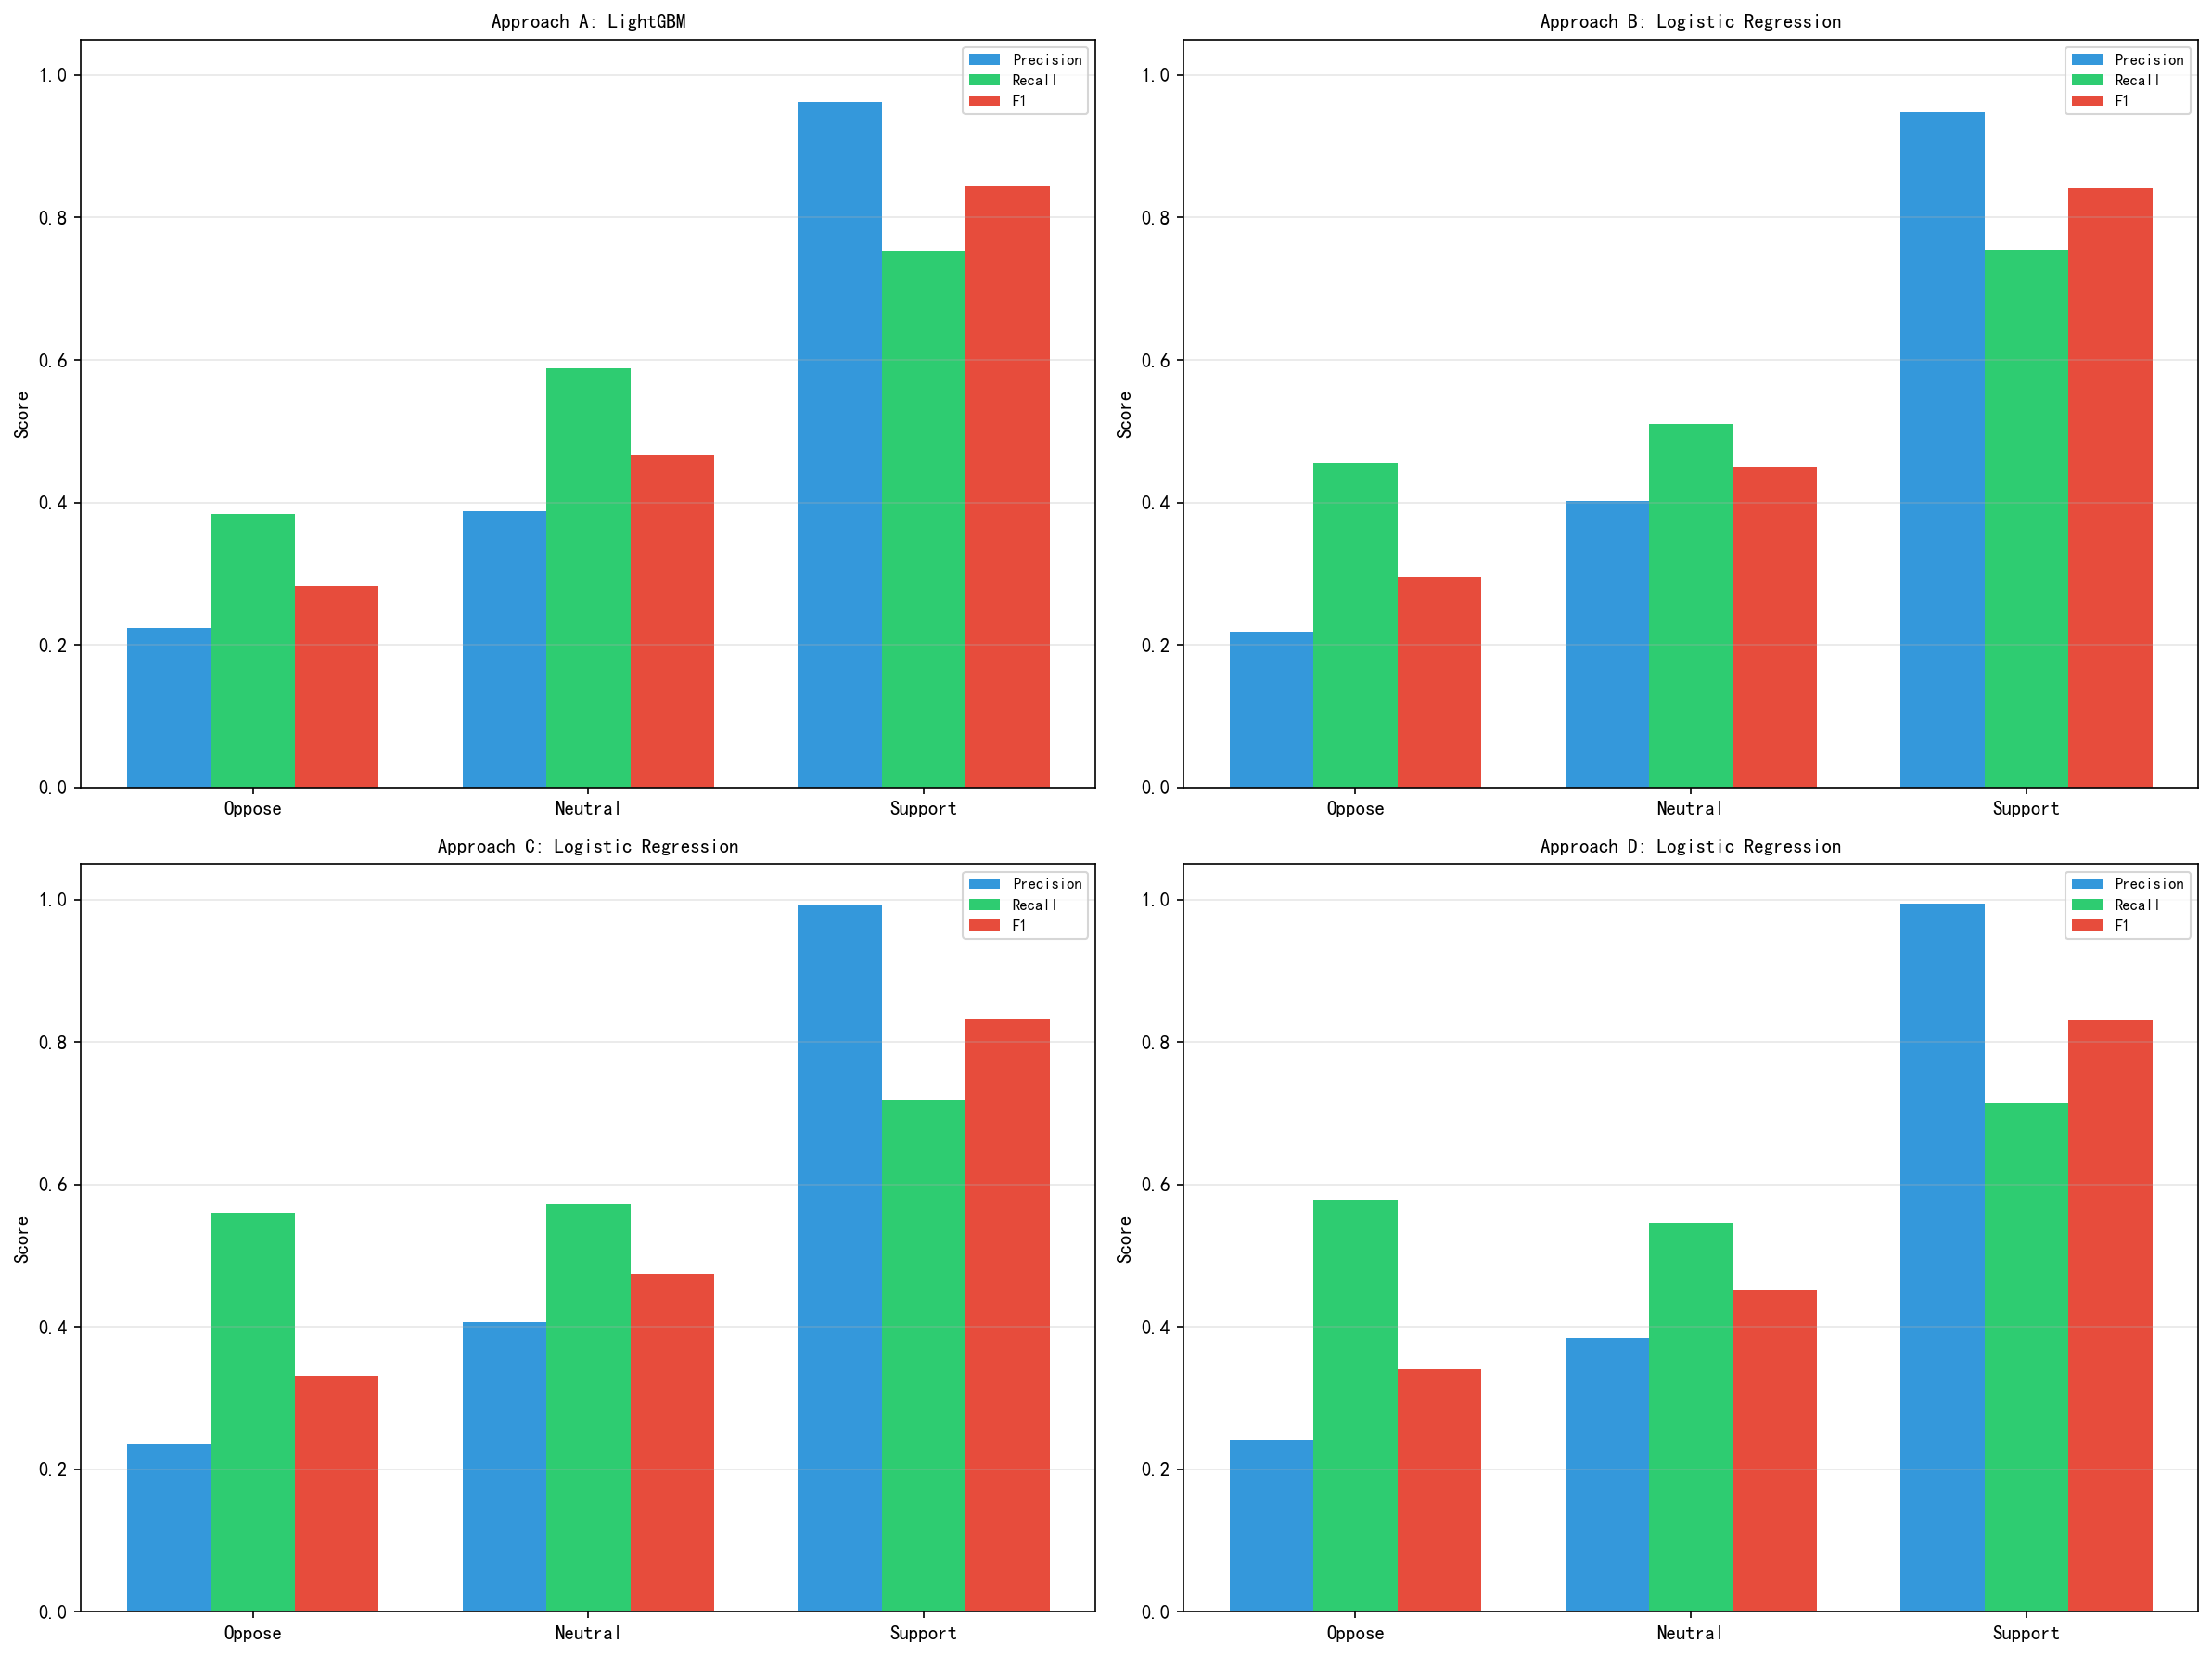
\includegraphics[width=0.95\textwidth]{figures/per_class_metrics.png}
    \caption{四种方案下最佳分类模型在三个类别上的精确率、召回率和F1得分。}
    \label{fig:per_class_metrics}
\end{figure}

\begin{figure}[H]
    \centering
    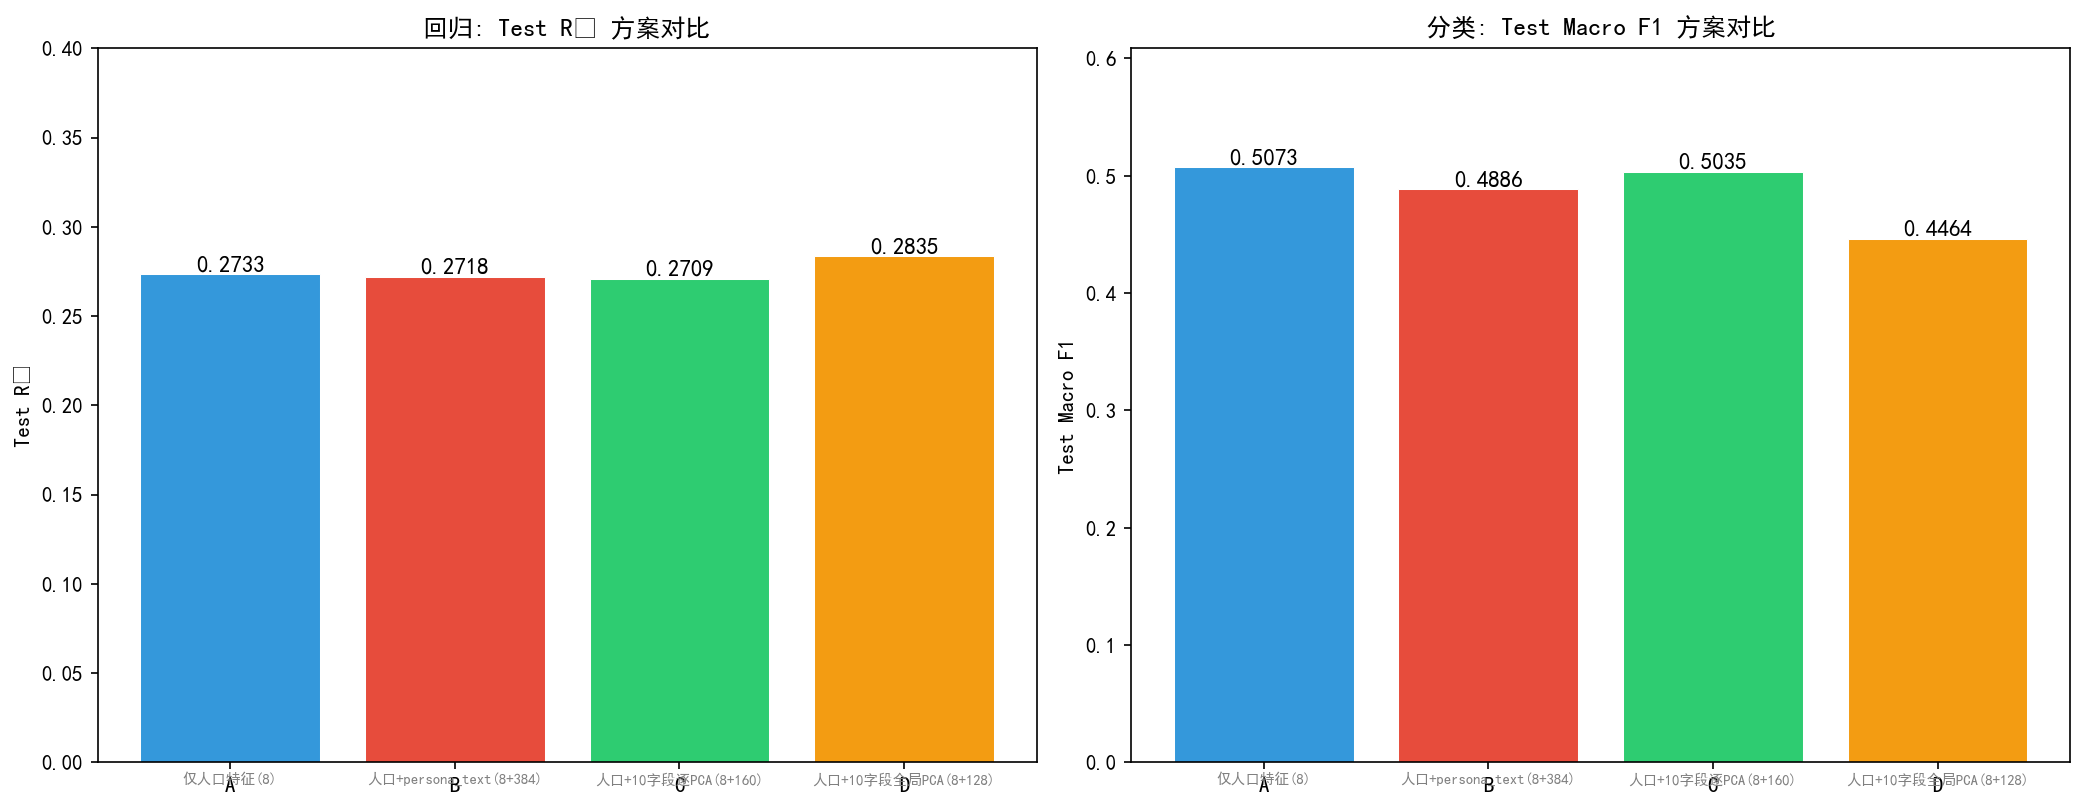
\includegraphics[width=0.95\textwidth]{figures/approach_comparison.png}
    \caption{四种特征方案在测试集上的表现对比。左：回归Test R$^2$；右：分类Test Macro F1。}
    \label{fig:approach_comparison}
\end{figure}

\begin{figure}[H]
    \centering
    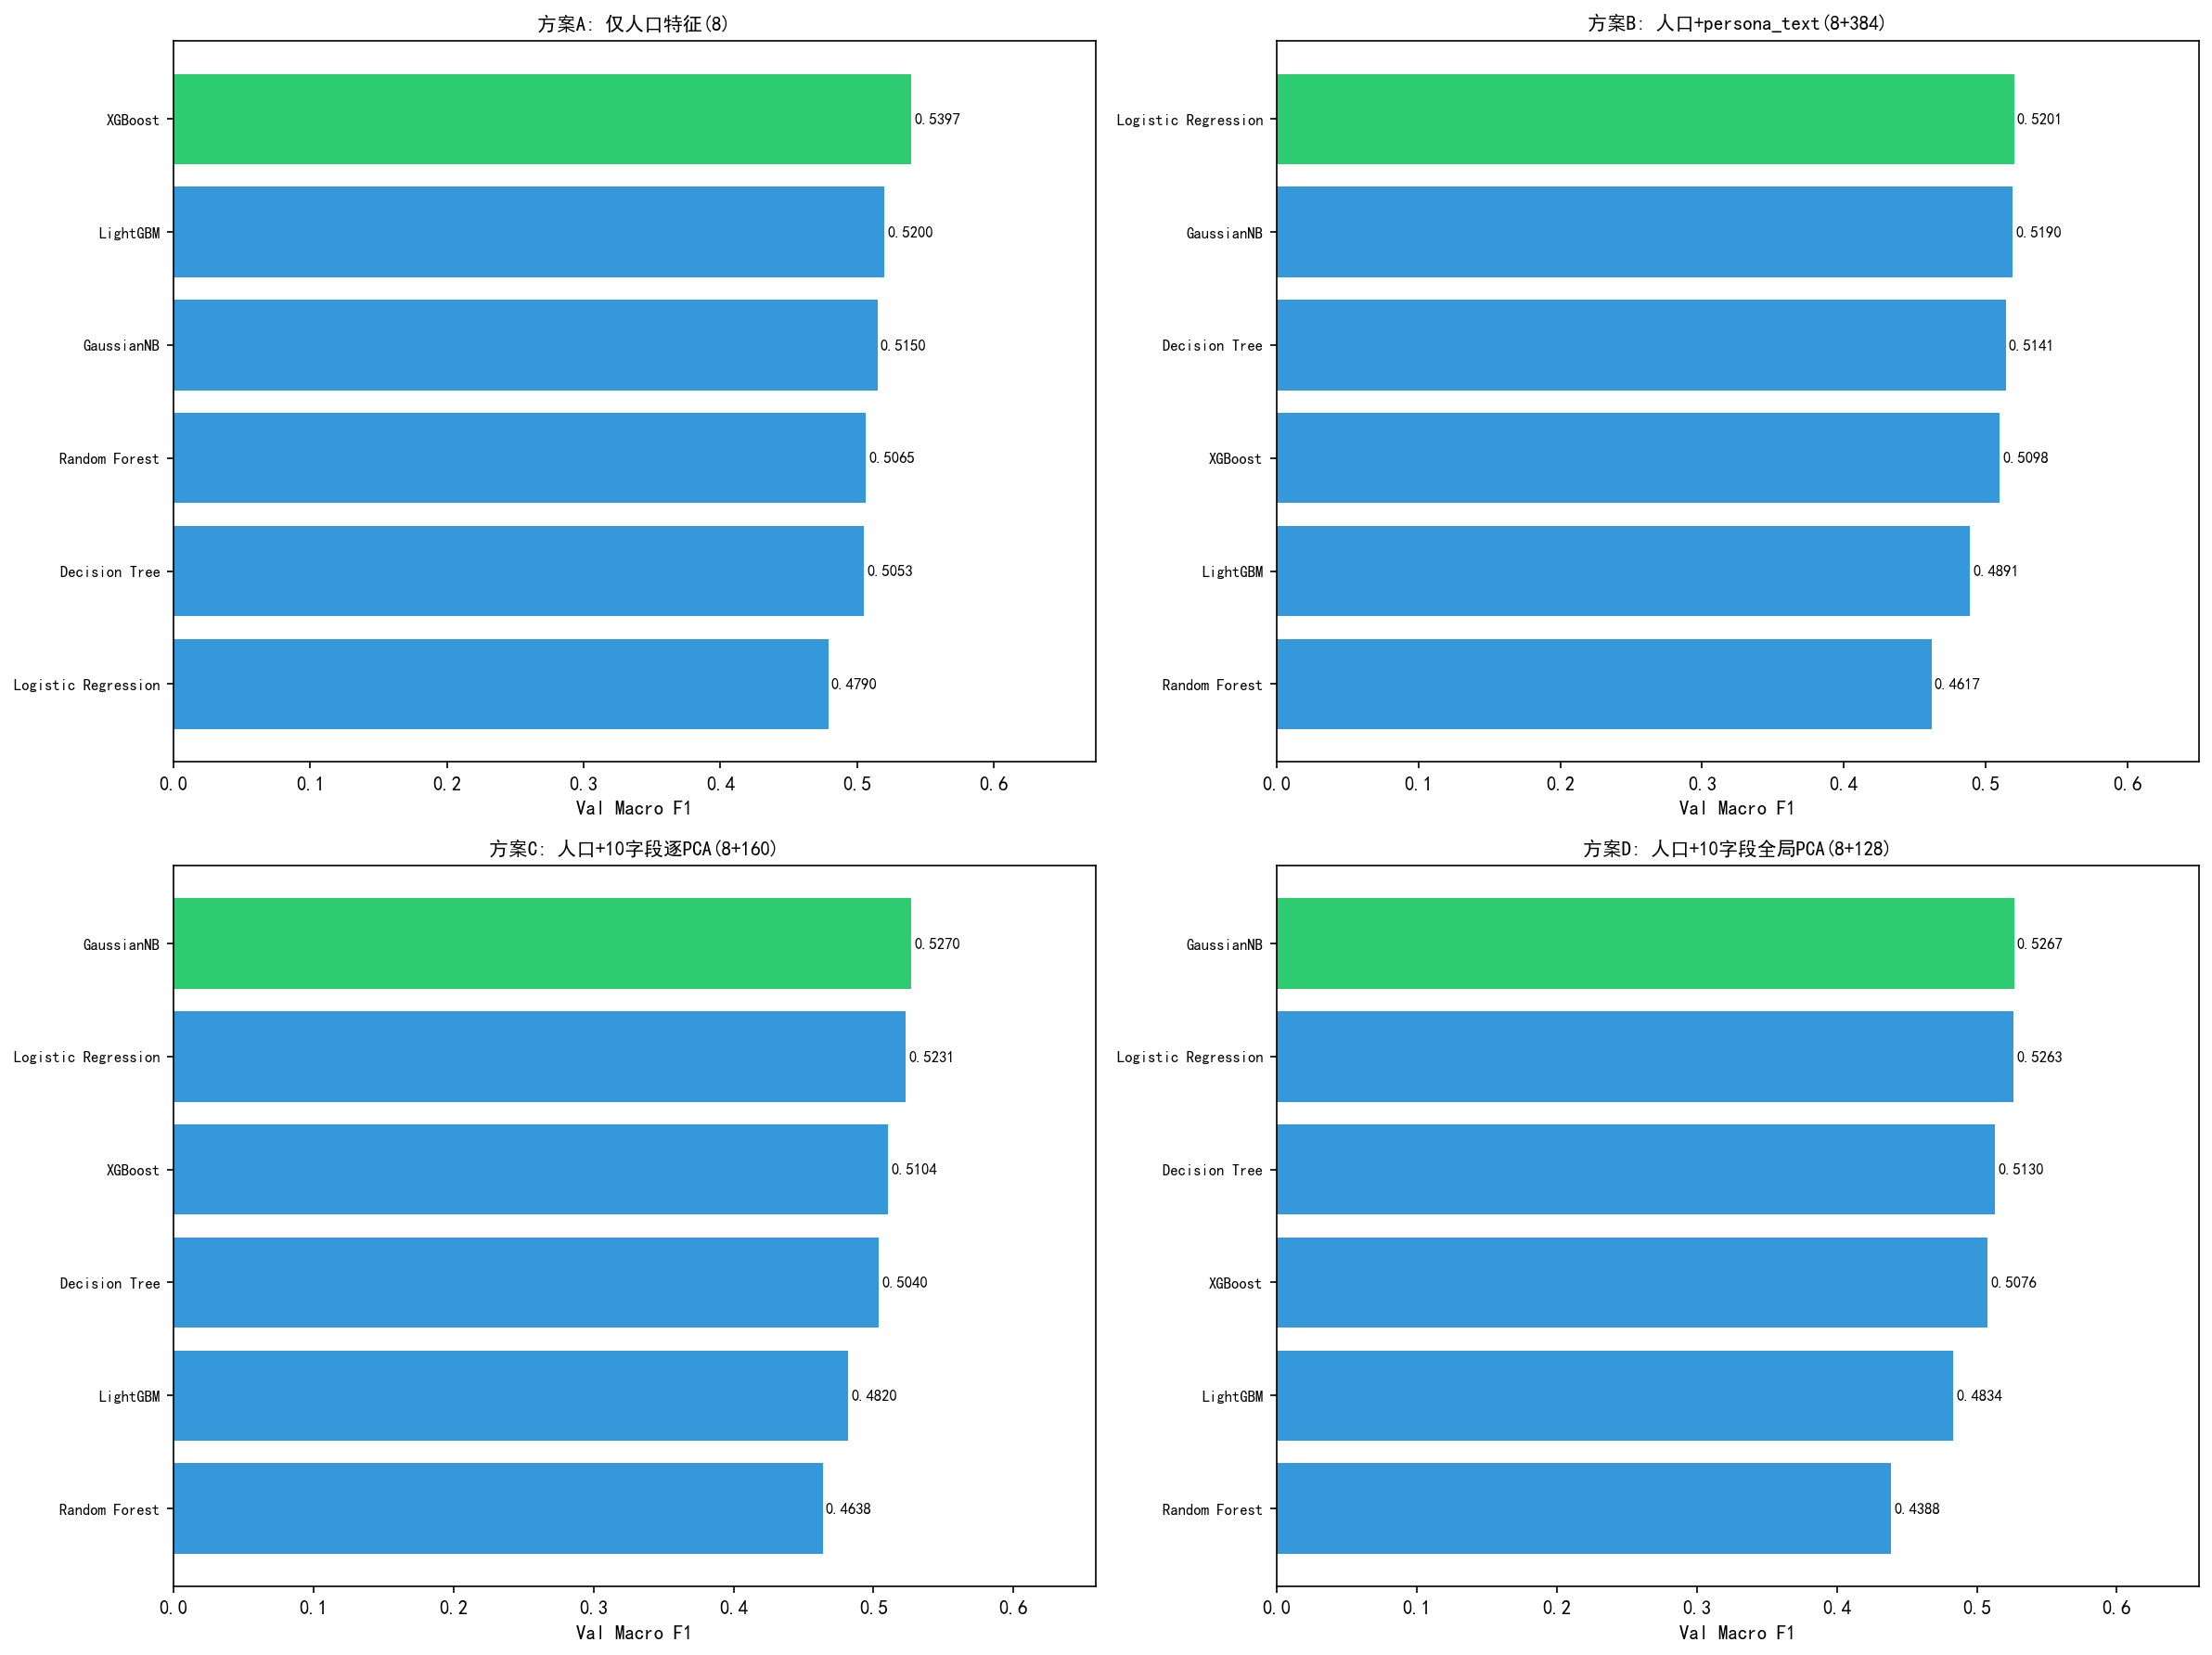
\includegraphics[width=0.95\textwidth]{figures/classification_by_approach.png}
    \caption{各方案各模型的分类Val Macro F1排名。}
    \label{fig:classification_by_approach}
\end{figure}

\begin{figure}[H]
    \centering
    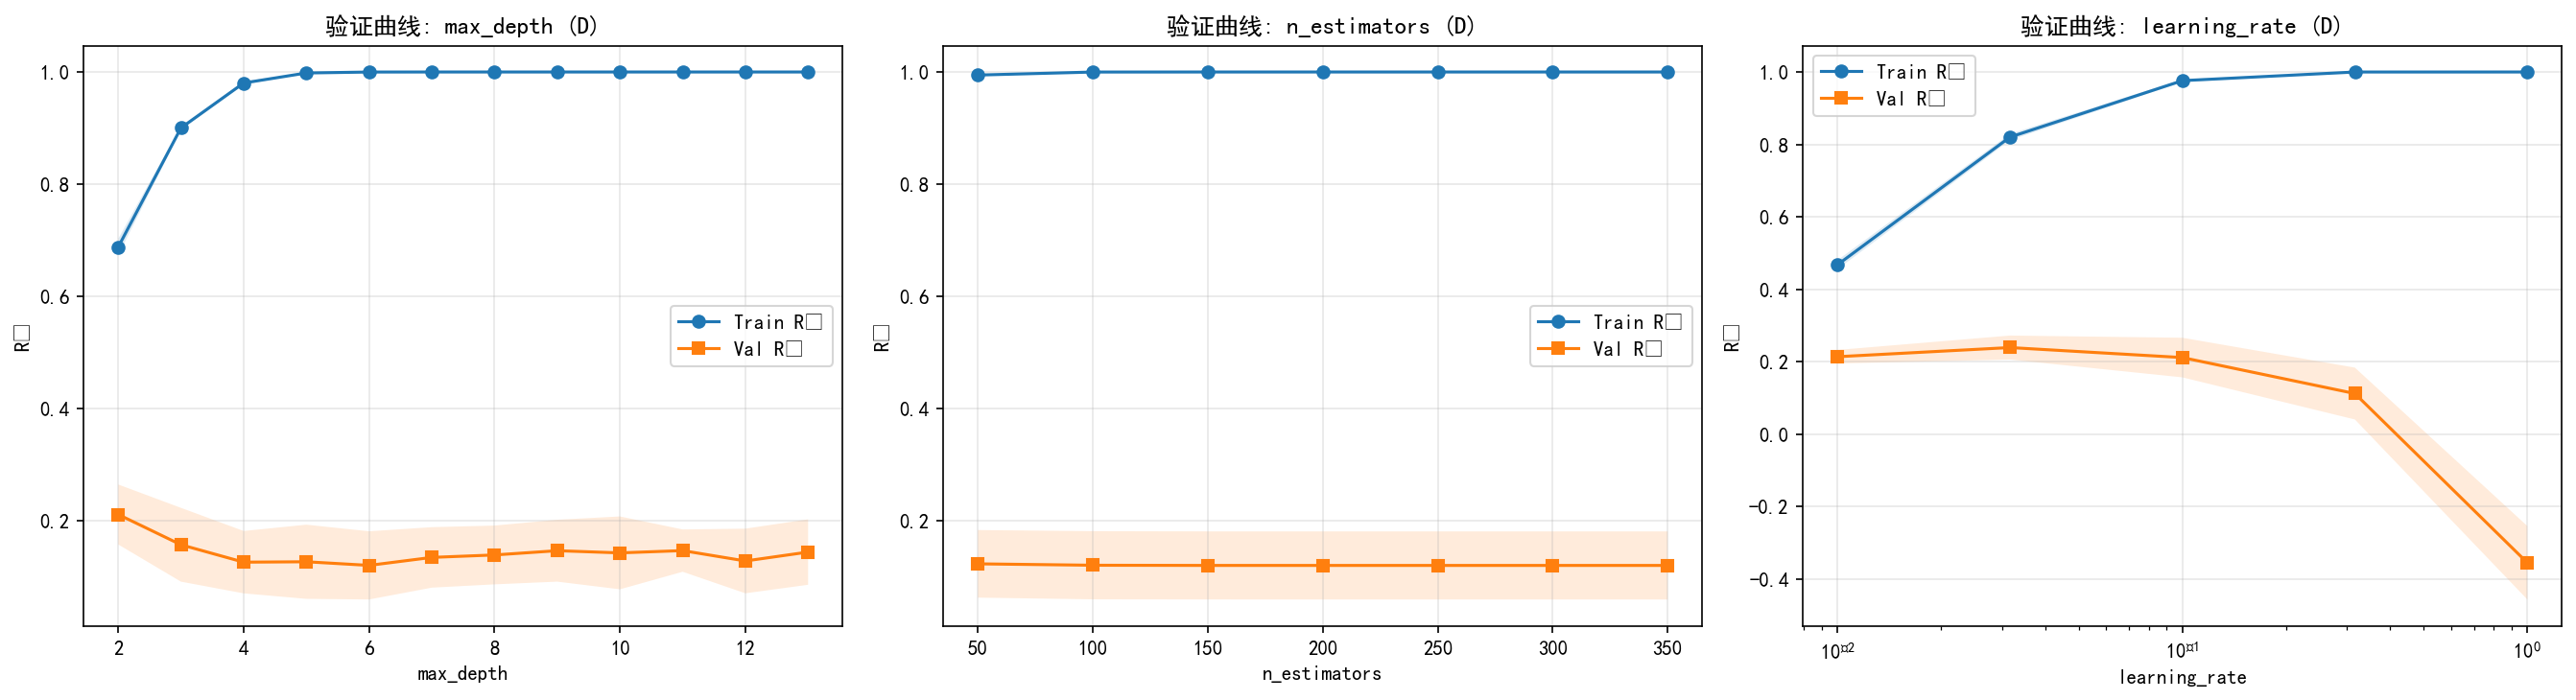
\includegraphics[width=0.95\textwidth]{figures/validation_curves.png}
    \caption{XGBoost超参数验证曲线（最佳方案）。}
    \label{fig:validation_curves}
\end{figure}

\end{document}
